% Options for packages loaded elsewhere
\PassOptionsToPackage{unicode}{hyperref}
\PassOptionsToPackage{hyphens}{url}
\PassOptionsToPackage{dvipsnames,svgnames,x11names}{xcolor}
%
\documentclass[
  a4paper,
]{scrreport}

\usepackage{amsmath,amssymb}
\usepackage{lmodern}
\usepackage{iftex}
\ifPDFTeX
  \usepackage[T1]{fontenc}
  \usepackage[utf8]{inputenc}
  \usepackage{textcomp} % provide euro and other symbols
\else % if luatex or xetex
  \usepackage{unicode-math}
  \defaultfontfeatures{Scale=MatchLowercase}
  \defaultfontfeatures[\rmfamily]{Ligatures=TeX,Scale=1}
\fi
% Use upquote if available, for straight quotes in verbatim environments
\IfFileExists{upquote.sty}{\usepackage{upquote}}{}
\IfFileExists{microtype.sty}{% use microtype if available
  \usepackage[]{microtype}
  \UseMicrotypeSet[protrusion]{basicmath} % disable protrusion for tt fonts
}{}
\makeatletter
\@ifundefined{KOMAClassName}{% if non-KOMA class
  \IfFileExists{parskip.sty}{%
    \usepackage{parskip}
  }{% else
    \setlength{\parindent}{0pt}
    \setlength{\parskip}{6pt plus 2pt minus 1pt}}
}{% if KOMA class
  \KOMAoptions{parskip=half}}
\makeatother
\usepackage{xcolor}
\setlength{\emergencystretch}{3em} % prevent overfull lines
\setcounter{secnumdepth}{5}
% Make \paragraph and \subparagraph free-standing
\ifx\paragraph\undefined\else
  \let\oldparagraph\paragraph
  \renewcommand{\paragraph}[1]{\oldparagraph{#1}\mbox{}}
\fi
\ifx\subparagraph\undefined\else
  \let\oldsubparagraph\subparagraph
  \renewcommand{\subparagraph}[1]{\oldsubparagraph{#1}\mbox{}}
\fi


\providecommand{\tightlist}{%
  \setlength{\itemsep}{0pt}\setlength{\parskip}{0pt}}\usepackage{longtable,booktabs,array}
\usepackage{calc} % for calculating minipage widths
% Correct order of tables after \paragraph or \subparagraph
\usepackage{etoolbox}
\makeatletter
\patchcmd\longtable{\par}{\if@noskipsec\mbox{}\fi\par}{}{}
\makeatother
% Allow footnotes in longtable head/foot
\IfFileExists{footnotehyper.sty}{\usepackage{footnotehyper}}{\usepackage{footnote}}
\makesavenoteenv{longtable}
\usepackage{graphicx}
\makeatletter
\def\maxwidth{\ifdim\Gin@nat@width>\linewidth\linewidth\else\Gin@nat@width\fi}
\def\maxheight{\ifdim\Gin@nat@height>\textheight\textheight\else\Gin@nat@height\fi}
\makeatother
% Scale images if necessary, so that they will not overflow the page
% margins by default, and it is still possible to overwrite the defaults
% using explicit options in \includegraphics[width, height, ...]{}
\setkeys{Gin}{width=\maxwidth,height=\maxheight,keepaspectratio}
% Set default figure placement to htbp
\makeatletter
\def\fps@figure{htbp}
\makeatother

\usepackage{venndiagram}
\newcommand{\NN}{\mathbb{N}}
\newcommand{\ZZ}{\mathbb{Z}}
\newcommand{\QQ}{\mathbb{Q}}
\newcommand{\RR}{\mathbb{R}}
\newcommand{\CC}{\mathbb{C}}
\DeclareMathOperator{\operatorname{Int}}{Int}
\DeclareMathOperator{\operatorname{Ext}}{Ext}
\DeclareMathOperator{\operatorname{Fr}}{Fr}
\DeclareMathOperator{\Adh}{Adh}
\DeclareMathOperator{\Ac}{Ac}
\DeclareMathOperator{\sen}{sen}
\makeatletter
\@ifpackageloaded{tcolorbox}{}{\usepackage[many]{tcolorbox}}
\@ifpackageloaded{fontawesome5}{}{\usepackage{fontawesome5}}
\definecolor{quarto-callout-color}{HTML}{909090}
\definecolor{quarto-callout-note-color}{HTML}{0758E5}
\definecolor{quarto-callout-important-color}{HTML}{CC1914}
\definecolor{quarto-callout-warning-color}{HTML}{EB9113}
\definecolor{quarto-callout-tip-color}{HTML}{00A047}
\definecolor{quarto-callout-caution-color}{HTML}{FC5300}
\definecolor{quarto-callout-color-frame}{HTML}{acacac}
\definecolor{quarto-callout-note-color-frame}{HTML}{4582ec}
\definecolor{quarto-callout-important-color-frame}{HTML}{d9534f}
\definecolor{quarto-callout-warning-color-frame}{HTML}{f0ad4e}
\definecolor{quarto-callout-tip-color-frame}{HTML}{02b875}
\definecolor{quarto-callout-caution-color-frame}{HTML}{fd7e14}
\makeatother
\makeatletter
\@ifpackageloaded{tikz}{}{\usepackage{tikz}}
\makeatother
\makeatletter
\@ifpackageloaded{bookmark}{}{\usepackage{bookmark}}
\makeatother
\makeatletter
\@ifpackageloaded{caption}{}{\usepackage{caption}}
\AtBeginDocument{%
\ifdefined\contentsname
  \renewcommand*\contentsname{Indice de contenidos}
\else
  \newcommand\contentsname{Indice de contenidos}
\fi
\ifdefined\listfigurename
  \renewcommand*\listfigurename{Listado de Figuras}
\else
  \newcommand\listfigurename{Listado de Figuras}
\fi
\ifdefined\listtablename
  \renewcommand*\listtablename{Listado de Tablas}
\else
  \newcommand\listtablename{Listado de Tablas}
\fi
\ifdefined\figurename
  \renewcommand*\figurename{Figura}
\else
  \newcommand\figurename{Figura}
\fi
\ifdefined\tablename
  \renewcommand*\tablename{Tabla}
\else
  \newcommand\tablename{Tabla}
\fi
}
\@ifpackageloaded{float}{}{\usepackage{float}}
\floatstyle{ruled}
\@ifundefined{c@chapter}{\newfloat{codelisting}{h}{lop}}{\newfloat{codelisting}{h}{lop}[chapter]}
\floatname{codelisting}{Listado}
\newcommand*\listoflistings{\listof{codelisting}{Listado de Listatdos}}
\usepackage{amsthm}
\theoremstyle{definition}
\newtheorem{exercise}{Ejercicio}[chapter]
\theoremstyle{remark}
\renewcommand*{\proofname}{Prueba}
\newtheorem*{remark}{Observación}
\newtheorem*{solution}{Solución}
\makeatother
\makeatletter
\@ifpackageloaded{caption}{}{\usepackage{caption}}
\@ifpackageloaded{subcaption}{}{\usepackage{subcaption}}
\makeatother
\makeatletter
\@ifpackageloaded{tcolorbox}{}{\usepackage[many]{tcolorbox}}
\makeatother
\makeatletter
\@ifundefined{shadecolor}{\definecolor{shadecolor}{rgb}{.97, .97, .97}}
\makeatother
\makeatletter
\makeatother
\ifLuaTeX
\usepackage[bidi=basic]{babel}
\else
\usepackage[bidi=default]{babel}
\fi
\babelprovide[main,import]{spanish}
% get rid of language-specific shorthands (see #6817):
\let\LanguageShortHands\languageshorthands
\def\languageshorthands#1{}
\ifLuaTeX
  \usepackage{selnolig}  % disable illegal ligatures
\fi
\IfFileExists{bookmark.sty}{\usepackage{bookmark}}{\usepackage{hyperref}}
\IfFileExists{xurl.sty}{\usepackage{xurl}}{} % add URL line breaks if available
\urlstyle{same} % disable monospaced font for URLs
\hypersetup{
  pdftitle={Problemas de Análisis Matemático},
  pdfauthor={Alfredo Sánchez Alberca},
  pdflang={es},
  colorlinks=true,
  linkcolor={blue},
  filecolor={Maroon},
  citecolor={Blue},
  urlcolor={Blue},
  pdfcreator={LaTeX via pandoc}}

\title{Problemas de Análisis Matemático}
\author{Alfredo Sánchez Alberca}
\date{1/6/2022}

\begin{document}
\begin{titlepage}

%\AddToShipoutPicture*{\put(0,0){\includegraphics[scale=0.8]{img/background2}}} % Imagen de fondo, requiere el paquete eso-pic.
\begin{center}
\vspace*{5cm}

\Huge
{\textbf{\textsf{Problemas de Análisis Matemático}}}

\vspace{0.5cm}
\LARGE
{\textbf{\textsf{}}}

\vspace{1.5cm}


\includegraphics[width=0.4\textwidth]{img/logos/infinito.png}
\end{center}

\vfill

\begin{flushleft}
\begin{tabular}{ll}
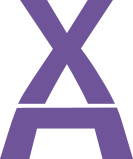
\includegraphics[width=0.1\textwidth]{img/logos/aprendeconalf.png} & \parbox[b]{5cm}{\Large\textsf{Alfredo
Sánchez
Alberca}\\ \textsf{asalber@ceu.es} \\ \textsf{https://aprendeconalf.es}}
\end{tabular}
\end{flushleft}
\end{titlepage}\ifdefined\Shaded\renewenvironment{Shaded}{\begin{tcolorbox}[interior hidden, borderline west={3pt}{0pt}{shadecolor}, enhanced, sharp corners, frame hidden, breakable, boxrule=0pt]}{\end{tcolorbox}}\fi

\renewcommand*\contentsname{Indice de contenidos}
{
\hypersetup{linkcolor=}
\setcounter{tocdepth}{2}
\tableofcontents
}
\bookmarksetup{startatroot}

\hypertarget{prefacio}{%
\chapter*{Prefacio}\label{prefacio}}
\addcontentsline{toc}{chapter}{Prefacio}

Colección de problemas de Análisis Matemático aplicado.

\bookmarksetup{startatroot}

\hypertarget{teoruxeda-de-conjuntos}{%
\chapter{Teoría de conjuntos}\label{teoruxeda-de-conjuntos}}

\leavevmode\vadjust pre{\hypertarget{exr-operaciones-conjuntos}{}}%
\begin{exercise}[]\label{exr-operaciones-conjuntos}

Dado el conjunto universo de los números de un dado
\(\Omega=\{1, 2, 3, 4, 5, 6\}\) y los subconjuntos correspondientes a
sacar par en el lanzamiento de un dado \(A=\{2, 4, 6\}\) y sacar menos
de 5 en el lanzamiento de un dado \(B=\{1, 2, 3, 4\}\), calcular e
interpretar los siguientes conjuntos:

\begin{enumerate}
\def\labelenumi{\alph{enumi}.}
\tightlist
\item
  \(A\cup B\)
\item
  \(A\cap B\)
\item
  \(\overline A\) y \(\overline B\)
\item
  \(A-B\) y \(B-A\)
\item
  \(A\triangle B\)
\item
  \(\overline{(A\cup B)}\)
\item
  \(\overline{(A\cap B)}\)
\item
  \(A\cup \overline B\)
\item
  \(\overline{\overline A \cap B}\)
\end{enumerate}

¿Qué conjuntos de números en el lanzamiento de un dado serían disjuntos
con \(A\)? ¿Y con \(A\cup B\)?

\end{exercise}

\begin{tcolorbox}[enhanced jigsaw, title=\textcolor{quarto-callout-tip-color}{\faLightbulb}\hspace{0.5em}{Solución}, colframe=quarto-callout-tip-color-frame, bottomrule=.15mm, breakable, arc=.35mm, opacityback=0, left=2mm, bottomtitle=1mm, titlerule=0mm, toptitle=1mm, rightrule=.15mm, opacitybacktitle=0.6, toprule=.15mm, colback=white, colbacktitle=quarto-callout-tip-color!10!white, leftrule=.75mm, coltitle=black]

\begin{enumerate}
\def\labelenumi{\alph{enumi}.}
\tightlist
\item
  \(A\cup B = \{1, 2, 3, 4, 6\}\)
\item
  \(A\cap B = \{2, 4\}\)
\item
  \(\overline A = \{1, 3, 5\}\) y \(\overline B = \{5, 6\}\)
\item
  \(A-B = \{6\}\) y \(B-A = \{1,3\}\)
\item
  \(A\triangle B = \{1, 3, 6\}\)
\item
  \(\overline{(A\cup B)} = \{5\}\)
\item
  \(\overline{(A\cap B)} = \{1,3, 5, 6\}\)
\item
  \(A\cup \overline B = \{2, 4, 5, 6\}\)
\item
  \(\overline{\overline A \cap B} = \{2, 4, 5, 6\}\)
\end{enumerate}

Serían disjuntos con \(A\) todos los conjuntos que solo tuviesen alguno
de los números \(1\), \(3\) o \(5\), por ejemplo el conjunto
\(\{1, 5\}\). El único conjunto disjunto con \(A\cup B\), además del
vacío es \(\{5\}\).

\end{tcolorbox}

\leavevmode\vadjust pre{\hypertarget{exr-expresion-conjuntos}{}}%
\begin{exercise}[]\label{exr-expresion-conjuntos}

Expresar con operaciones entre los conjuntos \(A\), \(B\) y \(C\), los
conjuntos que se corresponden con las regiones sombreadas en los
siguientes diagramas.

\end{exercise}

\begin{figure}

\begin{minipage}[t]{0.33\linewidth}

{\centering 

\raisebox{-\height}{

\begin{venndiagram3sets}[showframe=false,shade=blue!20]
\fillOnlyB
\fillCCapB
\end{venndiagram3sets}


}

\caption{a.}

}

\end{minipage}%
%
\begin{minipage}[t]{0.33\linewidth}

{\centering 

\raisebox{-\height}{

\usepackage{venndiagram}

\begin{venndiagram3sets}[showframe=false,shade=blue!20]
\fillOnlyA
\fillOnlyC
\fillACapB
\end{venndiagram3sets}


}

\caption{b.}

}

\end{minipage}%
%
\begin{minipage}[t]{0.33\linewidth}

{\centering 

\raisebox{-\height}{

\begin{venndiagram3sets}[showframe=false,shade=blue!20]
\fillOnlyA
\fillOnlyB
\fillOnlyC
\end{venndiagram3sets}


}

\caption{b.}

}

\end{minipage}%

\end{figure}

\begin{tcolorbox}[enhanced jigsaw, title=\textcolor{quarto-callout-tip-color}{\faLightbulb}\hspace{0.5em}{Solución}, colframe=quarto-callout-tip-color-frame, bottomrule=.15mm, breakable, arc=.35mm, opacityback=0, left=2mm, bottomtitle=1mm, titlerule=0mm, toptitle=1mm, rightrule=.15mm, opacitybacktitle=0.6, toprule=.15mm, colback=white, colbacktitle=quarto-callout-tip-color!10!white, leftrule=.75mm, coltitle=black]

\begin{enumerate}
\def\labelenumi{\alph{enumi}.}
\tightlist
\item
  \((B-A)\cup (A\cap B\cap C)\)
\item
  \((A\cup B)\cap \overline{(A\cap C)}\cap \overline{(B\cap C)}\cup (A\cap B\cap C)\)
\item
  \((A\cup B\cup C) - ((A\cap B)\cup (A\cap C)\cup (B\cap C))\)
\end{enumerate}

\end{tcolorbox}

\leavevmode\vadjust pre{\hypertarget{exr-leyes-morgan}{}}%
\begin{exercise}[]\label{exr-leyes-morgan}

Demostrar gráficamente las leyes de Morgan
\(\overline{A\cup B}=\overline A \cap \overline B\) y
\(\overline{A\cap B}=\overline A \cup \overline B\).

\end{exercise}

\leavevmode\vadjust pre{\hypertarget{exr-conjunto-potencia}{}}%
\begin{exercise}[]\label{exr-conjunto-potencia}

Construir por extensión el conjunto potencia del conjunto de los grupos
sanguíneos \(S=\{0, A, B, AB\}\). ¿Cuál es su cardinal?

\end{exercise}

\begin{tcolorbox}[enhanced jigsaw, title=\textcolor{quarto-callout-tip-color}{\faLightbulb}\hspace{0.5em}{Solución}, colframe=quarto-callout-tip-color-frame, bottomrule=.15mm, breakable, arc=.35mm, opacityback=0, left=2mm, bottomtitle=1mm, titlerule=0mm, toptitle=1mm, rightrule=.15mm, opacitybacktitle=0.6, toprule=.15mm, colback=white, colbacktitle=quarto-callout-tip-color!10!white, leftrule=.75mm, coltitle=black]
\begin{align*}
\mathcal{P}(S)&=\{\emptyset, \{A\}, \{B\}, \{AB\}, \\
& \{\emptyset,A\},\{\emptyset,B\}, \{\emptyset,AB\}, \{A,B\}, \{A,AB\}, \{B,AB\}, \{\emptyset,A,B\},\\ 
& \{\emptyset,A,AB\}, \{\emptyset,B,AB\}, \{A,B,AB\}, \\ 
& \{\emptyset,A,B,AB\} \}
\end{align*}
\end{tcolorbox}

\leavevmode\vadjust pre{\hypertarget{exr-producto-cartesiano-grupos-sanguineos}{}}%
\begin{exercise}[]\label{exr-producto-cartesiano-grupos-sanguineos}

Construir el producto cartesiano del conjunto d los grupos sanguíneos
\(S=\{0, A, B, AB\}\) y el conjunto de los factores Rh
\(R=\{\mbox{Rh}+, \mbox{Rh}-\}\).

\end{exercise}

\begin{tcolorbox}[enhanced jigsaw, title=\textcolor{quarto-callout-tip-color}{\faLightbulb}\hspace{0.5em}{Solución}, colframe=quarto-callout-tip-color-frame, bottomrule=.15mm, breakable, arc=.35mm, opacityback=0, left=2mm, bottomtitle=1mm, titlerule=0mm, toptitle=1mm, rightrule=.15mm, opacitybacktitle=0.6, toprule=.15mm, colback=white, colbacktitle=quarto-callout-tip-color!10!white, leftrule=.75mm, coltitle=black]
\begin{align*}
S \times R &=\{(0,\mbox{Rh}+), (0,\mbox{Rh}-), (A,\mbox{Rh}+)), (A,\mbox{Rh}-),\\
& (B,\mbox{Rh}+), (B,\mbox{Rh}-), (AB,\mbox{Rh}+), (AB,\mbox{Rh}-) \}
\end{align*}
\end{tcolorbox}

\leavevmode\vadjust pre{\hypertarget{exr-relacion-equivalencia-1}{}}%
\begin{exercise}[]\label{exr-relacion-equivalencia-1}

Demostrar que la relación
\(R=\{(x,y)\in \mathbb{Z}^2: x-y \mbox{ es par}\}\) es una relación de
equivalencia.

\end{exercise}

\begin{tcolorbox}[enhanced jigsaw, title=\textcolor{quarto-callout-tip-color}{\faLightbulb}\hspace{0.5em}{Solución}, colframe=quarto-callout-tip-color-frame, bottomrule=.15mm, breakable, arc=.35mm, opacityback=0, left=2mm, bottomtitle=1mm, titlerule=0mm, toptitle=1mm, rightrule=.15mm, opacitybacktitle=0.6, toprule=.15mm, colback=white, colbacktitle=quarto-callout-tip-color!10!white, leftrule=.75mm, coltitle=black]
\emph{Propiedad reflexiva}: \(\forall a\in\mathbb{Z}\) \(a-a=0\) es par,
de manera que \(aRa\).\\
\emph{Propiedad simétrica}: \(\forall a,b\in\mathbb{Z}\) si \(aRb\)
entonces \(a-b\) es par, es decir, existe \(k\in \mathbb{Z}\) tal que
\(a-b=2k\). Por tanto, \(b-a=2(-k)\) también es par y \(bRa\).
\emph{Propiedad transitiva}: \(\forall a,b,c\in\mathbb{Z}\), si \(aRb\)
y \(bRc\) entonces \(a-b\) y \(b-c\) son pares, de manera que su suma
\(a-b+b-c = a-c\) también es par, y \(aRc\).
\end{tcolorbox}

\leavevmode\vadjust pre{\hypertarget{exr-relaciones-equivalencia}{}}%
\begin{exercise}[]\label{exr-relaciones-equivalencia}

¿Cuáles de las siguientes relaciones son relaciones de equivalencia?
¿Cuáles don de orden?

\begin{enumerate}
\def\labelenumi{\alph{enumi}.}
\tightlist
\item
  \(R_1=\{(x,y)\in \mathbb{R}^2: x = y\}\)
\item
  \(R_2=\{(x,y)\in \mathbb{R}^2: x\leq y\}\)
\item
  \(R_3=\{(x,y)\in \mathbb{R}^2: x^2 + y^2 = 1\}\)
\item
  \(R_4=\{(x,y)\in \mathbb{R}^2: x^2 + y^2 \leq 1\}\)
\end{enumerate}

\end{exercise}

\begin{tcolorbox}[enhanced jigsaw, title=\textcolor{quarto-callout-tip-color}{\faLightbulb}\hspace{0.5em}{Solución}, colframe=quarto-callout-tip-color-frame, bottomrule=.15mm, breakable, arc=.35mm, opacityback=0, left=2mm, bottomtitle=1mm, titlerule=0mm, toptitle=1mm, rightrule=.15mm, opacitybacktitle=0.6, toprule=.15mm, colback=white, colbacktitle=quarto-callout-tip-color!10!white, leftrule=.75mm, coltitle=black]

\begin{enumerate}
\def\labelenumi{\alph{enumi}.}
\tightlist
\item
  \(R_1\) es relación de equivalencia.
\item
  \(R_2\) es relación de orden.
\item
  \(R_3\) no es relación de equivalencia ni de orden porque no cumple
  las propiedades reflexiva y transitiva.
\item
  \(R_4\) es no es relación de equivalencia ni de orden porque tampoco
  cumple las propiedades reflexiva y transitiva.
\end{enumerate}

\end{tcolorbox}

\leavevmode\vadjust pre{\hypertarget{exr-supremo-infimo-maximo-minimo}{}}%
\begin{exercise}[]\label{exr-supremo-infimo-maximo-minimo}

Para cada uno de los conjuntos siguientes, calcular si existe el
supremo, el ínfimo, el máximo y el mínimo.

\begin{enumerate}
\def\labelenumi{\alph{enumi}.}
\tightlist
\item
  \(A=\{1, 2, 3, 4, 5\}\)
\item
  \(B=\{x\in\mathbb{N} : x \mbox{ es par}\}\)
\item
  \(C=\{x\in\mathbb{Q} : 0< x \leq 1\}\)
\end{enumerate}

\end{exercise}

\begin{tcolorbox}[enhanced jigsaw, title=\textcolor{quarto-callout-tip-color}{\faLightbulb}\hspace{0.5em}{Solución}, colframe=quarto-callout-tip-color-frame, bottomrule=.15mm, breakable, arc=.35mm, opacityback=0, left=2mm, bottomtitle=1mm, titlerule=0mm, toptitle=1mm, rightrule=.15mm, opacitybacktitle=0.6, toprule=.15mm, colback=white, colbacktitle=quarto-callout-tip-color!10!white, leftrule=.75mm, coltitle=black]

\begin{enumerate}
\def\labelenumi{\alph{enumi}.}
\tightlist
\item
  \(\sup(A)=5\), \(\inf(A) = 1\), \(\max(A)=5\), \(\min(A)=1\).
\item
  \(\inf(B) = 2\) y \(\min(B)=2\). No existe el supremo ni el máximo
  porque \(B\) no está acotado superiormente.
\item
  \(\sup(C)=1\), \(\inf(C) = 0\) y \(\max(C)=1\). No existe el mínimo.
\end{enumerate}

\end{tcolorbox}

\leavevmode\vadjust pre{\hypertarget{exr-ejemplos-funciones}{}}%
\begin{exercise}[]\label{exr-ejemplos-funciones}

Dar ejemplos de funciones \(f:\mathbb{Z}\rightarrow \mathbb{Z}\) que
cumplan lo siguiente:

\begin{enumerate}
\def\labelenumi{\alph{enumi}.}
\tightlist
\item
  \(f\) es inyectiva pero no sobreyectiva.
\item
  \(f\) es sobreyectiva pero no inyectiva.
\item
  \(f\) no es inyectiva ni sobreyectiva.
\item
  \(f\) es biyectiva y distinta de la función identidad.
\end{enumerate}

\end{exercise}

\begin{tcolorbox}[enhanced jigsaw, title=\textcolor{quarto-callout-tip-color}{\faLightbulb}\hspace{0.5em}{Solución}, colframe=quarto-callout-tip-color-frame, bottomrule=.15mm, breakable, arc=.35mm, opacityback=0, left=2mm, bottomtitle=1mm, titlerule=0mm, toptitle=1mm, rightrule=.15mm, opacitybacktitle=0.6, toprule=.15mm, colback=white, colbacktitle=quarto-callout-tip-color!10!white, leftrule=.75mm, coltitle=black]

\begin{enumerate}
\def\labelenumi{\alph{enumi}.}
\tightlist
\item
  \(f(x)=2x\)
\item
  \(f(x)=x^3-x\).
\item
  \(f(x)=x^2\)
\item
  \(f(x)=2x+1\)
\end{enumerate}

\end{tcolorbox}

\leavevmode\vadjust pre{\hypertarget{exr-tipos-funciones}{}}%
\begin{exercise}[]\label{exr-tipos-funciones}

Dadas las siguientes funciones de \(\mathbb{R}\) en \(\mathbb{R}\),
estudiar cuáles son inyectivas y cuáles sobreyectivas:

\begin{enumerate}
\def\labelenumi{\alph{enumi}.}
\tightlist
\item
  \(f(x)=x^2\)
\item
  \(g(x)=x^3\)
\item
  \(h(x)=x^3-x^2-2x\)
\item
  \(i(x)=|x|\)
\end{enumerate}

\end{exercise}

\begin{tcolorbox}[enhanced jigsaw, title=\textcolor{quarto-callout-tip-color}{\faLightbulb}\hspace{0.5em}{Solución}, colframe=quarto-callout-tip-color-frame, bottomrule=.15mm, breakable, arc=.35mm, opacityback=0, left=2mm, bottomtitle=1mm, titlerule=0mm, toptitle=1mm, rightrule=.15mm, opacitybacktitle=0.6, toprule=.15mm, colback=white, colbacktitle=quarto-callout-tip-color!10!white, leftrule=.75mm, coltitle=black]

\begin{enumerate}
\def\labelenumi{\alph{enumi}.}
\tightlist
\item
  \(f(x)=x^2\) no es ni inyectiva ni sobreyectiva.
\item
  \(g(x)=x^3\) es biyectiva.
\item
  \(h(x)=x^3-x^2-2x\) es sobreyectiva pero no inyectiva.
\item
  \(i(x)=|x|\) no es ni inyectiva ni sobreyectiva.
\end{enumerate}

\end{tcolorbox}

\leavevmode\vadjust pre{\hypertarget{exr-composicion-funciones-inyectivas}{}}%
\begin{exercise}[]\label{exr-composicion-funciones-inyectivas}

Demostrar que la composición de dos funciones inyectivas es también
inyectiva.

\end{exercise}

\begin{tcolorbox}[enhanced jigsaw, title=\textcolor{quarto-callout-tip-color}{\faLightbulb}\hspace{0.5em}{Solución}, colframe=quarto-callout-tip-color-frame, bottomrule=.15mm, breakable, arc=.35mm, opacityback=0, left=2mm, bottomtitle=1mm, titlerule=0mm, toptitle=1mm, rightrule=.15mm, opacitybacktitle=0.6, toprule=.15mm, colback=white, colbacktitle=quarto-callout-tip-color!10!white, leftrule=.75mm, coltitle=black]
Sean \(f\) y \(g\) dos funciones inyectivas tales que
\(\operatorname{Im}(f)\subseteq\operatorname{Dom}(g)\). Veamos que
\(g\circ f\) es inyectiva. Supongamos ahora que existen
\(a, b\in \operatorname{Dom}(f)\) tales que \(g\circ f(a)=g\circ f(b)\),
es decir, \(g(f(a))=g(f(b))\). Como \(g\) es inyectiva, se tiene que
\(f(a)=f(b)\), y como \(f\) es inyectiva se tiene que \(a=b\), con lo
que \(g\circ f\) es inyectiva.
\end{tcolorbox}

\leavevmode\vadjust pre{\hypertarget{exr-cardinal-union-producto-cartesiano}{}}%
\begin{exercise}[]\label{exr-cardinal-union-producto-cartesiano}

Dados dos conjuntos finitos \(A\) y \(B\), demostrar que
\(|A\cup B| = |A|+|B|-|A\cap B|\) y que \(|A\times B|=|A||B|\).

\end{exercise}

\begin{tcolorbox}[enhanced jigsaw, title=\textcolor{quarto-callout-tip-color}{\faLightbulb}\hspace{0.5em}{Solución}, colframe=quarto-callout-tip-color-frame, bottomrule=.15mm, breakable, arc=.35mm, opacityback=0, left=2mm, bottomtitle=1mm, titlerule=0mm, toptitle=1mm, rightrule=.15mm, opacitybacktitle=0.6, toprule=.15mm, colback=white, colbacktitle=quarto-callout-tip-color!10!white, leftrule=.75mm, coltitle=black]

\begin{enumerate}
\def\labelenumi{\alph{enumi}.}
\item
  \(A\cup B = (A-B) \cup (B-A)\cup (A\cap B)\) con \((A-B)\),
  \(A\cup B\) y \(B-A\) disjuntos dos a dos, de manera que
  \(|A\cup B| = |A-B| + |B-A| + |A\cap B|\).

  Por otro lado, \(A=(A-B)\cup (A\cap B)\), y \(B=(B-A)\cup (A\cap B)\),
  de modo que

  \begin{align*}
   |A| + |B| - |A\cap B| &= |A-B| + |A\cap B| + |B-A| + |A\cap B| - |A\cap B| \\
   &= |A-B| + |B-A| + |A\cap B|,
   \end{align*}

  que coincide con el resultado anterior.
\item
  Supongamos que \(A=\{a_1,\ldots, a_n\}\) y \(B=\{b_1,\ldots, b_m\}\),
  de manera que \(|A|=n\) y \(|B|=m\). Para cada elemento \(a_i\in A\)
  se pueden formar \(m\) pares \((a_i,b_1),\ldots (a_i,b_m)\). Como
  \(A\) tiene \(n\) elementos, en total se pueden formar \(n\cdot m\)
  pares, así que \(|A\times B| = n\cdot m = |A||B|\).
\end{enumerate}

\end{tcolorbox}

\leavevmode\vadjust pre{\hypertarget{exr-cardinal-funcion-inyectiva-sobreyectiva}{}}%
\begin{exercise}[]\label{exr-cardinal-funcion-inyectiva-sobreyectiva}

Dada una función \(f:A\rightarrow B\), demostrar que si \(f\) es
inyectiva, entonces \(|A|\leq |B|\), y si \(f\) es sobreyectiva,
entonces \(|A|\geq |B|\). ¿Cómo es \(|A|\) en comparación con \(|B|\)
cuando \(f\) es biyectiva?

\end{exercise}

\begin{tcolorbox}[enhanced jigsaw, title=\textcolor{quarto-callout-tip-color}{\faLightbulb}\hspace{0.5em}{Solución}, colframe=quarto-callout-tip-color-frame, bottomrule=.15mm, breakable, arc=.35mm, opacityback=0, left=2mm, bottomtitle=1mm, titlerule=0mm, toptitle=1mm, rightrule=.15mm, opacitybacktitle=0.6, toprule=.15mm, colback=white, colbacktitle=quarto-callout-tip-color!10!white, leftrule=.75mm, coltitle=black]
Sea \(f:A\rightarrow B\) inyectiva. Entonces para cualesquiera
\(a_1,a_2\in A\) con \(a_1\neq a_2\) se tiene que \(f(a_1)\neq f(a_2)\),
por lo que \(|A|\leq |B|\).

Sea \(f:A\rightarrow B\) sobreyectiva. Entonces para todo \(b\in B\)
existe \(a\in A\) tal que \(f(a)=b\). Además dos elementos de \(B\) no
pueden tener la misma preimagen porque entonces \(f\) no sería una
función, por lo que \(|A|\geq |B|\).

De lo anterior se deduce que si \(f\) es biyectiva, entonces
\(|A|=|B|\).
\end{tcolorbox}

\leavevmode\vadjust pre{\hypertarget{exr-numero-funciones-inyectivas}{}}%
\begin{exercise}[]\label{exr-numero-funciones-inyectivas}

Dados dos conjuntos finitos \(A\) y \(B\) con \(|A|=n\) y \(|B|=m\).
¿Cuántas funciones distintas se pueden construir de \(A\) a \(B\). ¿Y
cuántas funciones inyectivas suponiendo que \(n\leq m\)?

\end{exercise}

\begin{tcolorbox}[enhanced jigsaw, title=\textcolor{quarto-callout-tip-color}{\faLightbulb}\hspace{0.5em}{Solución}, colframe=quarto-callout-tip-color-frame, bottomrule=.15mm, breakable, arc=.35mm, opacityback=0, left=2mm, bottomtitle=1mm, titlerule=0mm, toptitle=1mm, rightrule=.15mm, opacitybacktitle=0.6, toprule=.15mm, colback=white, colbacktitle=quarto-callout-tip-color!10!white, leftrule=.75mm, coltitle=black]
Se pueden construir \(m^n\) funciones distintas, y \(\frac{m!}{(m-n)!}\)
funciones inyectivas.
\end{tcolorbox}

\leavevmode\vadjust pre{\hypertarget{exr-ejemplo-conjunto-infinito-complemento}{}}%
\begin{exercise}[]\label{exr-ejemplo-conjunto-infinito-complemento}

Tomando el conjunto de los números naturales \(\mathbb{N}\) como
conjunto universo, dar un ejemplo de un subconjunto infinito cuyo
complemento también sea infinito.

\end{exercise}

\begin{tcolorbox}[enhanced jigsaw, title=\textcolor{quarto-callout-tip-color}{\faLightbulb}\hspace{0.5em}{Solución}, colframe=quarto-callout-tip-color-frame, bottomrule=.15mm, breakable, arc=.35mm, opacityback=0, left=2mm, bottomtitle=1mm, titlerule=0mm, toptitle=1mm, rightrule=.15mm, opacitybacktitle=0.6, toprule=.15mm, colback=white, colbacktitle=quarto-callout-tip-color!10!white, leftrule=.75mm, coltitle=black]
\(A=\{x\in\mathbb{N}: x \mbox{ es par}\}\) es infinito y
\(\overline A=\{x\in\mathbb{N}: x \mbox{ es impar}\}\) también es
infinito.
\end{tcolorbox}

\leavevmode\vadjust pre{\hypertarget{exr-subconjunto-infinito-numerable}{}}%
\begin{exercise}[]\label{exr-subconjunto-infinito-numerable}

Demostrar que todo conjunto infinito tiene un subconjunto infinito
numerable.

\end{exercise}

\begin{tcolorbox}[enhanced jigsaw, title=\textcolor{quarto-callout-tip-color}{\faLightbulb}\hspace{0.5em}{Solución}, colframe=quarto-callout-tip-color-frame, bottomrule=.15mm, breakable, arc=.35mm, opacityback=0, left=2mm, bottomtitle=1mm, titlerule=0mm, toptitle=1mm, rightrule=.15mm, opacitybacktitle=0.6, toprule=.15mm, colback=white, colbacktitle=quarto-callout-tip-color!10!white, leftrule=.75mm, coltitle=black]
Sean \(A\) un conjunto infinito. Como \(A\) no es vacío, existe un
elemento \(a_1\in A\). Considérese ahora el conjunto
\(A_1 = A\setminus \{a_1\}\). Es evidente que \(A_1\) sigue siendo
infinito y podemos elegir otro elemento \(a_2\in A_1\) de manera que el
conjunto \(A_2=A_1-\{a_2\}\) sigue siendo infinito. Repitiendo este
proceso indefinidamente obtenemos que el conjunto
\(\{a_1, a_2, \ldots\}\) es un subconjunto de \(A\) que es numerable.
\end{tcolorbox}

\leavevmode\vadjust pre{\hypertarget{exr-conjunto-equipotente-subconjunto}{}}%
\begin{exercise}[]\label{exr-conjunto-equipotente-subconjunto}

Demostrar que un conjunto es infinito si y solo si es equipotente a un
subconjunto propio.

\end{exercise}

\begin{tcolorbox}[enhanced jigsaw, title=\textcolor{quarto-callout-tip-color}{\faLightbulb}\hspace{0.5em}{Solución}, colframe=quarto-callout-tip-color-frame, bottomrule=.15mm, breakable, arc=.35mm, opacityback=0, left=2mm, bottomtitle=1mm, titlerule=0mm, toptitle=1mm, rightrule=.15mm, opacitybacktitle=0.6, toprule=.15mm, colback=white, colbacktitle=quarto-callout-tip-color!10!white, leftrule=.75mm, coltitle=black]
Sea \(A\) un conjunto. Si \(A\) es finito, entonces cualquier
subconjunto \(B\subset A\) cumple que \(|B| < |A|\) por lo que no se
puede establecer una biyección entre \(A\) y \(B\).

Si \(A\) es infinito, por el ejercicio anterior se tiene que existe un
subconjunto numerable \(B=\{a_1,a_2,\ldots\}\subseteq A\). Si tomamos la
aplicación \(f:B\to B\setminus\{a_1\}\) dada por \(f(a_i)=a_{i+1}\),
entonces \(f\) es biyectiva, y su extensión
\(\hat f: A\to A\setminus\{a_1\}\) dada por

\[
\hat f(x)=
\begin{cases}
x & \mbox{si } x\not\in B\\
f(x) & \mbox{si } x\in B
\end{cases}
\]

es también biyectiva, por lo que \(A\) es equipotente a
\(A\setminus \{a_1\}\) que es un subconjunto propio suyo.
\end{tcolorbox}

\leavevmode\vadjust pre{\hypertarget{exr-producto-cartesiano-numerable}{}}%
\begin{exercise}[]\label{exr-producto-cartesiano-numerable}

Demostrar que el producto cartesiano de dos conjuntos numerables es
numerable. ¿Y el producto cartesiano de \(n\) conjuntos numerables?

\end{exercise}

\begin{tcolorbox}[enhanced jigsaw, title=\textcolor{quarto-callout-tip-color}{\faLightbulb}\hspace{0.5em}{Solución}, colframe=quarto-callout-tip-color-frame, bottomrule=.15mm, breakable, arc=.35mm, opacityback=0, left=2mm, bottomtitle=1mm, titlerule=0mm, toptitle=1mm, rightrule=.15mm, opacitybacktitle=0.6, toprule=.15mm, colback=white, colbacktitle=quarto-callout-tip-color!10!white, leftrule=.75mm, coltitle=black]
Sean \(A\) y \(B\) dos conjuntos numerables. Entonces existe una
aplicación inyectiva \(f:A\to\mathbb{N}\) y otra \(g:B\to\mathbb{N}\).
Si se toma ahora la función \(h:A\times B\to \mathbb{N}\) definida como

\[ f(a,b) = 2^{f(a)}3^{g(b)}\, \forall a\in A, b\in B,\]

se tiene que \(f\) es inyectiva y por tanto \(A\times B\) es numerable.

Por inducción, es fácil probar que el producto cartesiano de \(n\)
conjuntos numerables es también numerable.
\end{tcolorbox}

\leavevmode\vadjust pre{\hypertarget{exr-racionales-numerables}{}}%
\begin{exercise}[]\label{exr-racionales-numerables}

Demostrar que el conjunto de los números racionales es numerable.

\end{exercise}

\begin{tcolorbox}[enhanced jigsaw, title=\textcolor{quarto-callout-tip-color}{\faLightbulb}\hspace{0.5em}{Solución}, colframe=quarto-callout-tip-color-frame, bottomrule=.15mm, breakable, arc=.35mm, opacityback=0, left=2mm, bottomtitle=1mm, titlerule=0mm, toptitle=1mm, rightrule=.15mm, opacitybacktitle=0.6, toprule=.15mm, colback=white, colbacktitle=quarto-callout-tip-color!10!white, leftrule=.75mm, coltitle=black]
Si se considera la aplicación
\(f:\mathbb{Q}\to \mathbb{Z}\times \mathbb{N}\) que a cada número
racional \(r\) le hace corresponder el par
\((p,q)\in \mathbb{Z}\times \mathbb{N}\) donde \(\frac{p}{q}\) es la
fracción irreducible de \(r\) con denominador positivo, se tiene que
\(f\) es inyectiva. Como el producto cartesiano de dos conjuntos
numerables es numerable, existe otra aplicación inyectiva de
\(g:\mathbb{Z}\times \mathbb{N}\to \mathbb{N}\), con lo que
\(g\circ f:\mathbb{Q}\to\mathbb{N}\) es inyectiva y \(\mathbb{Q}\) es
numerable.
\end{tcolorbox}

\leavevmode\vadjust pre{\hypertarget{exr-union-numerables}{}}%
\begin{exercise}[]\label{exr-union-numerables}

Demostrar que la unión de dos conjuntos numerables es numerable.

\end{exercise}

\begin{tcolorbox}[enhanced jigsaw, title=\textcolor{quarto-callout-tip-color}{\faLightbulb}\hspace{0.5em}{Solución}, colframe=quarto-callout-tip-color-frame, bottomrule=.15mm, breakable, arc=.35mm, opacityback=0, left=2mm, bottomtitle=1mm, titlerule=0mm, toptitle=1mm, rightrule=.15mm, opacitybacktitle=0.6, toprule=.15mm, colback=white, colbacktitle=quarto-callout-tip-color!10!white, leftrule=.75mm, coltitle=black]
Sean \(A\) y \(B\) dos conjuntos numerables disjuntos. Entonces existen
dos biyecciones \(f:A\to \mathbb{N}\) y \(g:B\to \mathbb{N}\). A partir
de estas biyecciones se puede definir otra \(h:A\cup B\to \mathbb{N}\)
dada por

\[h(x)=
\begin{cases}
2f(x)-1 & \mbox{si } x\in A\\
2g(x) & \mbox{si } x\in B
\end{cases}
\]

Así pues, \(A\cup B\) es numerable.

Si \(A\) y \(B\) no son disjuntos, entonces
\(A\cup B=A\cup (B\setminus A)\). Si
\(B\setminus A=\{b_1,\ldots, b_n\}\) es finito, se puede tomar la
biyección \(g=\{(b_1,1),\ldots,(b_n,n)\}\) y, a partir de ella,
construir la biyección \(h:A\cup B\to \mathbb{N}\) dada por

\[h(x)=
\begin{cases}
f(x)+n & \mbox{si } x\in A\\
g(x) & \mbox{si } x\in B\setminus A
\end{cases}
\]

Mientras que si \(B\setminus A\) es infinito, se puede razonar como al
principio pues \(A\) y \(B\setminus A\) son disjuntos.
\end{tcolorbox}

\leavevmode\vadjust pre{\hypertarget{exr-irracionales-no-numerables}{}}%
\begin{exercise}[]\label{exr-irracionales-no-numerables}

Demostrar que el conjunto de los números irracionales no es numerable.

\end{exercise}

\begin{tcolorbox}[enhanced jigsaw, title=\textcolor{quarto-callout-tip-color}{\faLightbulb}\hspace{0.5em}{Solución}, colframe=quarto-callout-tip-color-frame, bottomrule=.15mm, breakable, arc=.35mm, opacityback=0, left=2mm, bottomtitle=1mm, titlerule=0mm, toptitle=1mm, rightrule=.15mm, opacitybacktitle=0.6, toprule=.15mm, colback=white, colbacktitle=quarto-callout-tip-color!10!white, leftrule=.75mm, coltitle=black]
Ya hemos visto en el ejercicio Ejercicio~\ref{exr-racionales-numerables}
que \(\mathbb{Q}\) es numerable, de manera que si
\(\mathbb{R}\setminus \mathbb{Q}\) fuese numerable, entonces por el
Ejercicio~\ref{exr-union-numerables}
\(\mathbb{Q}\cup \mathbb{R}\setminus \mathbb{Q}=\mathbb{R}\) sería
numerable, lo cual no es cierto.
\end{tcolorbox}

\leavevmode\vadjust pre{\hypertarget{exr-union-numerable-conjuntos-numerables}{}}%
\begin{exercise}[]\label{exr-union-numerable-conjuntos-numerables}

Demostrar la unión de un conjunto numerable de conjuntos numerables es
numerable.

\end{exercise}

\begin{tcolorbox}[enhanced jigsaw, title=\textcolor{quarto-callout-tip-color}{\faLightbulb}\hspace{0.5em}{Solución}, colframe=quarto-callout-tip-color-frame, bottomrule=.15mm, breakable, arc=.35mm, opacityback=0, left=2mm, bottomtitle=1mm, titlerule=0mm, toptitle=1mm, rightrule=.15mm, opacitybacktitle=0.6, toprule=.15mm, colback=white, colbacktitle=quarto-callout-tip-color!10!white, leftrule=.75mm, coltitle=black]
Sea \(A\) un conjunto numerable de conjuntos numerables. Por ser \(A\)
numerable existe una biyección \(f:\mathbb{N}\to A\), de manera que
podemos enumerar los elementos de \(A\) de tal forma que \(A_i=f(i)\).
Del mismo modo, como cada conjunto \(A_i\) es numerable se puede
establecer una enumeración de sus elementos
\(A_i=\{a_{i1},a_{i2},\ldots\}\). Así pues, podemos representar los
elementos de \(\cup_{i=1}^\infty A_i\) en una tabla como la siguiente

\[
\begin{array}{cccccc}
a_{11} & \rightarrow & a_{12} & & a_{13} & \ldots \\
& \swarrow & & \nearrow & \downarrow \\
a_{21} & & a_{22} & & a_{23} & \ldots \\
\downarrow & \nearrow & & \swarrow \\
a_{31} & & a_{32} & & a_{33} & \ldots \\
\vdots & & \vdots & & \vdots & \ddots
\end{array}
\]

Siguiendo el orden de las flechas es posible enumerar todos los
elementos de este conjunto, por lo que \(\cup_{i=1}^\infty A_i\) es
numerable.
\end{tcolorbox}

\leavevmode\vadjust pre{\hypertarget{exr-conjunto-polinomios-no-numerable}{}}%
\begin{exercise}[]\label{exr-conjunto-polinomios-no-numerable}

Demostrar que el conjunto de todos los polinomios con coeficientes
enteros
\(P=\{a_0+a_1x+a_2x^2+\cdots+a_nx^n: n\in \mathbb{N}, a_i\in \mathbb{Z}\}\)
es numerable. ¿Y el de los polinomios con coeficientes racionales?

\end{exercise}

\begin{tcolorbox}[enhanced jigsaw, title=\textcolor{quarto-callout-tip-color}{\faLightbulb}\hspace{0.5em}{Solución}, colframe=quarto-callout-tip-color-frame, bottomrule=.15mm, breakable, arc=.35mm, opacityback=0, left=2mm, bottomtitle=1mm, titlerule=0mm, toptitle=1mm, rightrule=.15mm, opacitybacktitle=0.6, toprule=.15mm, colback=white, colbacktitle=quarto-callout-tip-color!10!white, leftrule=.75mm, coltitle=black]
Para cada \(n\in\mathbb{N}\) sea \(P_n\) el conjunto de los polinomios
de grado \(n\) con coeficientes enteros
\(P_n=\{a_0+a_1x+a_2x^2+\cdots+a_nx^n: a_i\in \mathbb{Z}\}\). Para cada
polinomio \(a_0+a_1x+a_2x^2+\cdots+a_nx^n\in P_n\) podemos establecer
una biyección entre sus coeficientes y la tupla
\(p_n=(a_0,a_1,\ldots,a_n)\), con \(a_i\in\mathbb{Z}\). Por tanto,
existe una biyección entre \(P_n\) y \(\mathbb{Z}^n\), y como
\(\mathbb{Z}^n\) es numerable, el \(P_n\) también lo es.

Finalmente, \(P=\cup_{i=1}^\infty P_n\) que es la unión numerable de
conjuntos numerables, que, como ya se vió en el
Ejercicio~\ref{exr-union-numerable-conjuntos-numerables}, es numerable.
\end{tcolorbox}

\leavevmode\vadjust pre{\hypertarget{exr-conjuntos-numerables}{}}%
\begin{exercise}[]\label{exr-conjuntos-numerables}

¿Cuáles de los siguientes conjuntos son numerables?

\begin{enumerate}
\def\labelenumi{\alph{enumi}.}
\tightlist
\item
  \(A=\{3k: k\in \mathbb{Z}\}\)
\item
  \(B=\{x\in \mathbb{Q}: -10 < x < 10\}\)
\item
  \(C = \{x\in \mathbb{R}: 0\leq x\leq 1\}\)
\item
  \(D=\{(x,y): x\in \mathbb{Z}, y\in \mathbb{Q}\}\)
\item
  \(E=\{1/n : n\in \mathbb{N}\}\)
\end{enumerate}

\end{exercise}

\leavevmode\vadjust pre{\hypertarget{exr-conjunto-secuencias-adn-numerable}{}}%
\begin{exercise}[]\label{exr-conjunto-secuencias-adn-numerable}

¿Es el conjunto de todas las secuencias infinitas de ADN numerable?

\end{exercise}

\bookmarksetup{startatroot}

\hypertarget{nuxfameros-reales}{%
\chapter{Números reales}\label{nuxfameros-reales}}

\leavevmode\vadjust pre{\hypertarget{exr-supremos-infimos-reales}{}}%
\begin{exercise}[]\label{exr-supremos-infimos-reales}

Para los siguientes subconjuntos de números reales, determinar si están
acotados por arriba o por abajo, y en tal caso dar el supremo o el
ínfimo.

\begin{enumerate}
\def\labelenumi{\alph{enumi}.}
\tightlist
\item
  \(A = \{-1,0,1\}\)
\item
  \(B= [0,1)\)
\item
  \(C= (0,\infty)\)
\item
  \(D= \left\{1+\frac{1}{n}:n\in\mathbb{N}\right\}\)
\item
  \(E= \left\{(-2)^n:n\in\mathbb{N}\right\}\)
\item
  \(F= \{x\in\mathbb{R}:x^2-3x+2=0\}\)
\item
  \(G= \{x\in\mathbb{R}:x^3-x<0\}\)
\end{enumerate}

\end{exercise}

\begin{tcolorbox}[enhanced jigsaw, title=\textcolor{quarto-callout-tip-color}{\faLightbulb}\hspace{0.5em}{Solución}, colframe=quarto-callout-tip-color-frame, bottomrule=.15mm, breakable, arc=.35mm, opacityback=0, left=2mm, bottomtitle=1mm, titlerule=0mm, toptitle=1mm, rightrule=.15mm, opacitybacktitle=0.6, toprule=.15mm, colback=white, colbacktitle=quarto-callout-tip-color!10!white, leftrule=.75mm, coltitle=black]

\begin{enumerate}
\def\labelenumi{\alph{enumi}.}
\item
  \(A\) está acotado por arriba y por abajo. \(\sup(A)=1\) y
  \(\inf(A)=-1\).
\item
  \(B\) está acotado por arriba y por abajo. \(\sup(B)=1\) y
  \(\inf(B)=0\).
\item
  \(C\) está acotado por abajo, pero no por arriba. \(\inf(C)=0\).
\item
  \(D\) está acotado por arriba y por abajo. \(\sup(D)=2\) y
  \(\inf(D)=1\).
\item
  \(E\) no está acotado por arriba ni por abajo.
\item
  \(F\) está acotado por arriba y por abajo.\(\sup(F)=2\) y
  \(\inf(F)=1\).
\item
  \(G\) está acotado por arriba pero no por abajo. \(\sup(G)=1\).
\end{enumerate}

\end{tcolorbox}

\leavevmode\vadjust pre{\hypertarget{exr-supremo-infimo-maximo-minimo-2}{}}%
\begin{exercise}[]\label{exr-supremo-infimo-maximo-minimo-2}

Calcular el supremo y el ínfimo de los siguientes conjuntos. ¿Tienen
máximo y mínimo?

\begin{enumerate}
\def\labelenumi{\alph{enumi}.}
\tightlist
\item
  \(A=\{x\in \mathbb{R} : 2 < x^2-2 < 7\}\)
\item
  \(B=\{x\in \mathbb{R} : 1 < 4x^2 - 3 \leq 5\}\)
\end{enumerate}

\end{exercise}

\begin{tcolorbox}[enhanced jigsaw, title=\textcolor{quarto-callout-tip-color}{\faLightbulb}\hspace{0.5em}{Solución}, colframe=quarto-callout-tip-color-frame, bottomrule=.15mm, breakable, arc=.35mm, opacityback=0, left=2mm, bottomtitle=1mm, titlerule=0mm, toptitle=1mm, rightrule=.15mm, opacitybacktitle=0.6, toprule=.15mm, colback=white, colbacktitle=quarto-callout-tip-color!10!white, leftrule=.75mm, coltitle=black]

\begin{enumerate}
\def\labelenumi{\alph{enumi}.}
\item
  \(A=(-3,-2)\cup(2,3)\), que como está acotado tiene supremo
  \(\sup(A)=3\) e ínfimo \(\inf(A)=-3\). Sin embargo, \(3\not \in A\) y
  \(-3\not\in A\), por lo que no tiene ni máximo ni mínimo.
\item
  \(B=[-\sqrt{2},-1)\cup(1,\sqrt{2}]\), que como está acotado tiene
  supremo \(\sup(B)=\sqrt{2}\) e ínfimo \(\inf(B)=-\sqrt{2}\). Como
  además, \(-\sqrt{2} \in B\) y \(\sqrt{2}\in B\), se tiene que
  \(\max(B)=\sqrt{2}\) y \(\min(B)=-\sqrt{2}\).
\end{enumerate}

\end{tcolorbox}

\leavevmode\vadjust pre{\hypertarget{exr-supremo-funciones}{}}%
\begin{exercise}[]\label{exr-supremo-funciones}

Dadas dos funciones \(f\) y \(g\) ambas con dominio
\(A\subseteq \mathbb{R}\), demostrar que si sus imágenes están acotadas
y \(f(a)\leq g(a)\) \(\forall a\in A\), entonces
\(\sup(\operatorname{Im}(f))\leq \sup(\operatorname{Im}(g))\).

\end{exercise}

\begin{tcolorbox}[enhanced jigsaw, title=\textcolor{quarto-callout-tip-color}{\faLightbulb}\hspace{0.5em}{Solución}, colframe=quarto-callout-tip-color-frame, bottomrule=.15mm, breakable, arc=.35mm, opacityback=0, left=2mm, bottomtitle=1mm, titlerule=0mm, toptitle=1mm, rightrule=.15mm, opacitybacktitle=0.6, toprule=.15mm, colback=white, colbacktitle=quarto-callout-tip-color!10!white, leftrule=.75mm, coltitle=black]
Como las imágenes de \(f\) y \(g\) están acotadas, y suponiendo que no
fuesen vacías, por el axioma del supremo, se tiene que existe
\(c,d\in\mathbb{R}\) tales que \(c=\sup(\operatorname{Im}(f))\) y
\(d= \sup(\operatorname{Im}(g))\). Como \(d\) es el supremo de la imagen
de \(g\), se tiene que es una cota superior de la imagen de \(f\), ya
que, para cualquier \(a\in A\), se tiene \(f(a)\leq g(a)\leq d\). Por
consiguiente, tiene que ser \(c\leq d\), ya que de lo contrario \(c\) no
sería el supremo por ser \(d\) una cota superior de la imagen de \(f\)
menor que \(c\).
\end{tcolorbox}

\leavevmode\vadjust pre{\hypertarget{exr-cotas-conjunto-opuestos}{}}%
\begin{exercise}[]\label{exr-cotas-conjunto-opuestos}

Demostrar que si \(c\in\mathbb{R}\) es una cota superior de un conjunto
\(A\), entonces \(-c\) es una cota inferior del conjunto de los opuestos
\(A'=\{-a\in\mathbb{R}: a\in A\}\), y si \(c\) es una cota inferior de
\(A\) entonces \(-c\) es una cota superior de \(A'\).

\end{exercise}

\begin{tcolorbox}[enhanced jigsaw, title=\textcolor{quarto-callout-tip-color}{\faLightbulb}\hspace{0.5em}{Solución}, colframe=quarto-callout-tip-color-frame, bottomrule=.15mm, breakable, arc=.35mm, opacityback=0, left=2mm, bottomtitle=1mm, titlerule=0mm, toptitle=1mm, rightrule=.15mm, opacitybacktitle=0.6, toprule=.15mm, colback=white, colbacktitle=quarto-callout-tip-color!10!white, leftrule=.75mm, coltitle=black]
Sea \(c\in\mathbb{R}\) una cota superior del conjunto \(A\). Entonces,
\(a\leq c\) \(\forall a\in A\). De ello se deduce que para cualquier
\(a\in A\),

\[
a<c \Rightarrow (-1)a\geq (-1)c \Rightarrow -a\geq -c, 
\]

lo que demuestra que \(-c\) es una cota inferior de \(A'\).

Del mismo modo, si \(c\) una cota inferior del conjunto \(A\). Entonces,
\(c\leq a\) \(\forall a\in A\), y de ello se deduce que para cualquier
\(a\in A\),

\[
c<a \Rightarrow (-1)c\geq (-1)a \Rightarrow -c\geq -a, 
\]

de manera que \(-c\) es cota superior de \(A'\).
\end{tcolorbox}

\leavevmode\vadjust pre{\hypertarget{exr-propiedad-infimo}{}}%
\begin{exercise}[]\label{exr-propiedad-infimo}

Demostrar que todo subconjunto no vacío de números reales acotado
inferiormente tiene un ínfimo.

\end{exercise}

\begin{tcolorbox}[enhanced jigsaw, title=\textcolor{quarto-callout-tip-color}{\faLightbulb}\hspace{0.5em}{Solución}, colframe=quarto-callout-tip-color-frame, bottomrule=.15mm, breakable, arc=.35mm, opacityback=0, left=2mm, bottomtitle=1mm, titlerule=0mm, toptitle=1mm, rightrule=.15mm, opacitybacktitle=0.6, toprule=.15mm, colback=white, colbacktitle=quarto-callout-tip-color!10!white, leftrule=.75mm, coltitle=black]
Sea \(A\subset\mathbb{R}\) no vacío y acotado inferiormente. Entonces
existe un \(c\in\mathbb{R}\) que es cota inferior de \(A\). Si tomamos
ahora el conjunto \(A'=\{-a\in\mathbb{R}: a\in A\}\), por el ejercicio
Ejercicio~\ref{exr-cotas-conjunto-opuestos}, se cumple que \(-c\) es una
cota superior de \(A'\). Así pues, \(A'\) es un conjunto no vacío y
acotado superiormente, y por el axioma del supremo, existe
\(-s\in\mathbb{R}\) tal que \(-s=\sup(A')\).

Veamos ahora que \(s\) es el ínfimo de \(A\). Como \(-s\) es el supremo
de \(A'\), es una cota superior de \(A'\), y por el ejercicio
Ejercicio~\ref{exr-cotas-conjunto-opuestos}, se cumple que \(-(-s)=s\)
es cota inferior de \(A\). Supongamos ahora que existe otra cota
inferior \(x\) de \(A\) tal que \(x>s\). Entonces, aplicando una vez más
el Ejercicio~\ref{exr-cotas-conjunto-opuestos}, se tiene que \(-x\) es
cota superior de \(A'\), pero
\(x>s\Rightarrow (-1)x<(-1)s \Rightarrow -x<-s\), lo que contradice que
\(-s\) sea el supremo de \(A'\), ya que \(-x\) sería una cota superior
menor que \(-s\). Luego \(s\) es el ínfimo de \(A\).
\end{tcolorbox}

\leavevmode\vadjust pre{\hypertarget{exr-propiedad-valor-absoluto}{}}%
\begin{exercise}[]\label{exr-propiedad-valor-absoluto}

Demostrar que \(|a|-|b|\leq |a-b|\) \(\forall a,b\in\mathbb{R}\).

\end{exercise}

\begin{tcolorbox}[enhanced jigsaw, title=\textcolor{quarto-callout-tip-color}{\faLightbulb}\hspace{0.5em}{Solución}, colframe=quarto-callout-tip-color-frame, bottomrule=.15mm, breakable, arc=.35mm, opacityback=0, left=2mm, bottomtitle=1mm, titlerule=0mm, toptitle=1mm, rightrule=.15mm, opacitybacktitle=0.6, toprule=.15mm, colback=white, colbacktitle=quarto-callout-tip-color!10!white, leftrule=.75mm, coltitle=black]

Veamos todas las posibilidades que pueden darse:

\begin{itemize}
\tightlist
\item
  Si \(a=0\), entonces \(|a|-|b|= -|b|\leq |-b| = |a-b|\).
\item
  Si \(b=0\), entonces \(|a|-|b|=|a|= |a-b|\).
\item
  Si \(a\geq b>0\), entonces \(|a|-|b|=a-b=|a-b|\).
\item
  Si \(b\geq a>0\), entonces \(|a|-|b|=a-b\leq 0\leq |a-b|\).
\item
  Si \(a>0>b\), entonces \(|a|-|b| = a-(-b) =a+b < a-b =|a-b|\).
\item
  Si \(b>0>a\), entonces \(|a|-|b| = -a-b < -a+b = -(a-b) = |a-b|\).
\item
  Si \(a\leq b<0\), entonces
  \(|a|-|b| = -a-(-b) = -a+b = -(a-b) = |a-b|\).
\item
  Si \(b\leq a<0\), entonces
  \(|a|-|b| = -a-(-b) = -a+b \leq 0 \leq |a-b|\).
\end{itemize}

\end{tcolorbox}

\leavevmode\vadjust pre{\hypertarget{exr-propiedad-arquimediana-1}{}}%
\begin{exercise}[]\label{exr-propiedad-arquimediana-1}

Usando la propiedad arquimediana de los números reales, demostrar que
para cualquier número real \(a\in\mathbb{R}\) con \(a>0\) existe un
número natural \(n\) tal que \(n-1\leq a< n\).

\end{exercise}

\begin{tcolorbox}[enhanced jigsaw, title=\textcolor{quarto-callout-tip-color}{\faLightbulb}\hspace{0.5em}{Solución}, colframe=quarto-callout-tip-color-frame, bottomrule=.15mm, breakable, arc=.35mm, opacityback=0, left=2mm, bottomtitle=1mm, titlerule=0mm, toptitle=1mm, rightrule=.15mm, opacitybacktitle=0.6, toprule=.15mm, colback=white, colbacktitle=quarto-callout-tip-color!10!white, leftrule=.75mm, coltitle=black]
Como \(a>0\) se tiene que \(\frac{1}{a}>0\), y por la propiedad
arquimediana se cumple que existe \(n\in \mathbb{N}\) tal que \(a<n\).

Considérese ahora el conjunto \(A=\{m\in \mathbb{N}: a<m\}\). Como
\(a<n\) se tiene que \(n\in A\) y por tanto \(A\) no está vacío.
Aplicando ahora el principio de buena ordenación de los números
naturales, como \(A\subset \mathbb{N}\), existe un primer elemento
\(n_0\in A\), tal que \(n_0-1\not\in A\), de manera que \(n_0-1\leq a\)
y con ello se tiene que \$\(n_0-1\leq a<n\).
\end{tcolorbox}

\leavevmode\vadjust pre{\hypertarget{exr-densidad-racionales}{}}%
\begin{exercise}[]\label{exr-densidad-racionales}

Se dice que un conjunto \(A\) es denso en \(\mathbb{R}\) si cada
intervalo \((a,b)\) de \(\mathbb{R}\) contiene algún elemento de \(A\).
Demostrar que \(\mathbb{Q}\) es denso en \(\mathbb{R}\).

\end{exercise}

\begin{tcolorbox}[enhanced jigsaw, title=\textcolor{quarto-callout-tip-color}{\faLightbulb}\hspace{0.5em}{Solución}, colframe=quarto-callout-tip-color-frame, bottomrule=.15mm, breakable, arc=.35mm, opacityback=0, left=2mm, bottomtitle=1mm, titlerule=0mm, toptitle=1mm, rightrule=.15mm, opacitybacktitle=0.6, toprule=.15mm, colback=white, colbacktitle=quarto-callout-tip-color!10!white, leftrule=.75mm, coltitle=black]
La prueba es la misma que la de la propiedad arquimediana. Basta con
tomar \(n\in \mathbb{N}\) tal que \(\frac{1}{n}< b-a\). Si ahora se toma
el primer múltiplo de \(1/n\) tal que \(a<\frac{m}{n}\), también se
cumplirá que \(\frac{m}{n}<b\), ya que de lo contrario
\(\frac{m-1}{n}<a<b<\frac{m}{n}\) lo que lleva a la contradicción de que
\(\frac{1}{n}>b-a\).
\end{tcolorbox}

\bookmarksetup{startatroot}

\hypertarget{topologuxeda-de-los-nuxfameros-reales}{%
\chapter{Topología de los números
reales}\label{topologuxeda-de-los-nuxfameros-reales}}

\leavevmode\vadjust pre{\hypertarget{exr-sucesion-intervalos-anidados}{}}%
\begin{exercise}[]\label{exr-sucesion-intervalos-anidados}

Dada la sucesión de intervalos anidados \(I_n=[0,\frac{1}{n}]\),
\(n\in\mathbb{N}\), demostrar que \(\cap_{n=1}^\infty I_n= \{0\}\).
Demostrar también que si se consideran intervalos abiertos en lugar de
cerrados entonces la intersección es vacía.

\end{exercise}

\begin{tcolorbox}[enhanced jigsaw, title=\textcolor{quarto-callout-tip-color}{\faLightbulb}\hspace{0.5em}{Solución}, colframe=quarto-callout-tip-color-frame, bottomrule=.15mm, breakable, arc=.35mm, opacityback=0, left=2mm, bottomtitle=1mm, titlerule=0mm, toptitle=1mm, rightrule=.15mm, opacitybacktitle=0.6, toprule=.15mm, colback=white, colbacktitle=quarto-callout-tip-color!10!white, leftrule=.75mm, coltitle=black]
En primer lugar, es fácil ver que \(0\in\cap_{n=1}^\infty I_n\) ya que
\(0\in I_n\) \(\forall n\in\mathbb{N}\). Veamos ahora que \(0\) es el
único elemento de la intersección. Para cualquier \(x>0\), aplicando la
propiedad arquimediana se tiene que existe \(n\in\mathbb{N}\) tal que
\(\frac{1}{n}<x\), de manera que \(x\not\in [0,\frac{1}{n}]=I_n\), por
lo que \(x\not\in\cap_{n=1}^\infty I_n\). Por tanto,
\(\cap_{n=1}^\infty I_n=\{0\}\).

Si se consideran intervalos abiertos en lugar de cerrados, entonces
\(0\) tampoco pertenecería a la intersección y
\(\cap_{n=1}^\infty I_n=\emptyset\).
\end{tcolorbox}

\leavevmode\vadjust pre{\hypertarget{exr-interior-conjunto-unitario}{}}%
\begin{exercise}[]\label{exr-interior-conjunto-unitario}

¿Cuál es el interior del conjunto \(A=\{a\}\)?

\end{exercise}

\begin{tcolorbox}[enhanced jigsaw, title=\textcolor{quarto-callout-tip-color}{\faLightbulb}\hspace{0.5em}{Solución}, colframe=quarto-callout-tip-color-frame, bottomrule=.15mm, breakable, arc=.35mm, opacityback=0, left=2mm, bottomtitle=1mm, titlerule=0mm, toptitle=1mm, rightrule=.15mm, opacitybacktitle=0.6, toprule=.15mm, colback=white, colbacktitle=quarto-callout-tip-color!10!white, leftrule=.75mm, coltitle=black]
\(a\) no es un punto interior de \(A\), ya que para cualquier
\(\varepsilon>0\), el entorno
\((a-\varepsilon, a+\varepsilon)\not\subseteq A\). Por tanto,
\(\operatorname{Int}(A)=\emptyset\).

En general, cualquier conjunto con un solo punto no tiene puntos
interiores.
\end{tcolorbox}

\leavevmode\vadjust pre{\hypertarget{exr-interior-exterior-frontera}{}}%
\begin{exercise}[]\label{exr-interior-exterior-frontera}

Sean \(a,b,c\in\mathbb{R}\) tales que \(a<b<c\) y sea
\(A=\{a\}\cup (b,c)\). Calcular \(\operatorname{Int}(A)\),
\(\operatorname{Ext}(A)\) y \(\operatorname{Fr}(A)\).

\end{exercise}

\begin{tcolorbox}[enhanced jigsaw, title=\textcolor{quarto-callout-tip-color}{\faLightbulb}\hspace{0.5em}{Solución}, colframe=quarto-callout-tip-color-frame, bottomrule=.15mm, breakable, arc=.35mm, opacityback=0, left=2mm, bottomtitle=1mm, titlerule=0mm, toptitle=1mm, rightrule=.15mm, opacitybacktitle=0.6, toprule=.15mm, colback=white, colbacktitle=quarto-callout-tip-color!10!white, leftrule=.75mm, coltitle=black]
Como el interior de un conjunto con un solo punto es vacío y el interior
de un intervalo abierto es el propio intervalo abierto (ver
\href{https://aprendeconalf.es/analisis-manual/topologia-reales.html\#prp-interior-intervalo-abierto}{proposición}),
se tiene que \(\operatorname{Int}(A)=(a,b)\). Por otro lado,
\(\overline{A}=(-\infty,a)\cup (a,b)\cup (c,\infty)\), que al ser la
unión de intervalos abiertos se tiene que
\(\operatorname{Ext}(A)=\operatorname{Int}(\overline{A})=(-\infty,a)\cup (a,b)\cup (c,\infty)\).
Finalmente, \(\operatorname{Fr}(A)=\{a,b,c\}\), ya que cualquier entorno
de estos puntos contiene puntos de \(A\) y de \(\overline{A}\).
\end{tcolorbox}

\leavevmode\vadjust pre{\hypertarget{exr-frontera-enteros}{}}%
\begin{exercise}[]\label{exr-frontera-enteros}

Demostrar que todos los puntos de \(\mathbb{Z}\) son puntos frontera.

\end{exercise}

\begin{tcolorbox}[enhanced jigsaw, title=\textcolor{quarto-callout-tip-color}{\faLightbulb}\hspace{0.5em}{Solución}, colframe=quarto-callout-tip-color-frame, bottomrule=.15mm, breakable, arc=.35mm, opacityback=0, left=2mm, bottomtitle=1mm, titlerule=0mm, toptitle=1mm, rightrule=.15mm, opacitybacktitle=0.6, toprule=.15mm, colback=white, colbacktitle=quarto-callout-tip-color!10!white, leftrule=.75mm, coltitle=black]
Sea \(x\in\mathbb{Z}\), entonces, para cualquier \(\varepsilon>0\), el
entorno \((x-\varepsilon, x+\varepsilon)\) siempre contiene números
enteros (por ejemplo el propio \(x\)), y números no enteros, por los que
\(x\) es un punto frontera.
\end{tcolorbox}

\leavevmode\vadjust pre{\hypertarget{exr-interior-racionales-irracionales}{}}%
\begin{exercise}[]\label{exr-interior-racionales-irracionales}

Demostrar que el conjunto de los números racionales no tiene puntos
interiores. ¿Y el conjunto de los números irracionales?

\end{exercise}

\begin{tcolorbox}[enhanced jigsaw, title=\textcolor{quarto-callout-tip-color}{\faLightbulb}\hspace{0.5em}{Solución}, colframe=quarto-callout-tip-color-frame, bottomrule=.15mm, breakable, arc=.35mm, opacityback=0, left=2mm, bottomtitle=1mm, titlerule=0mm, toptitle=1mm, rightrule=.15mm, opacitybacktitle=0.6, toprule=.15mm, colback=white, colbacktitle=quarto-callout-tip-color!10!white, leftrule=.75mm, coltitle=black]
Sea \(x\in\mathbb{Q}\), entonces, para cualquier \(\varepsilon>0\), por
la
\href{https://aprendeconalf.es/analisis-manual/cuerpo-reales.html\#thm-densidad-racionales}{densidad
de los números racionales}, el entorno
\((x-\varepsilon, x+\varepsilon)\) siempre contiene números racionales,
y por la
\href{https://aprendeconalf.es/analisis-manual/cuerpo-reales.html\#thm-densidad-irracionales}{densidad
de los números irracionales} también contiene números irracionales, de
manera que todos los puntos de \(\mathbb{Q}\) son frontera y no tiene
puntos interiores.

Por el mismo motivo, \(\mathbb{R}\setminus\mathbb{Q}\) tampoco tiene
puntos interiores y todos sus puntos son puntos frontera.
\end{tcolorbox}

\leavevmode\vadjust pre{\hypertarget{exr-interior-subconjunto}{}}%
\begin{exercise}[]\label{exr-interior-subconjunto}

Demostrar que si \(x\) es un punto interior de \(A\) y \(A\subseteq B\),
entonces \(x\) también es un punto interior de \(B\).

\end{exercise}

\begin{tcolorbox}[enhanced jigsaw, title=\textcolor{quarto-callout-tip-color}{\faLightbulb}\hspace{0.5em}{Solución}, colframe=quarto-callout-tip-color-frame, bottomrule=.15mm, breakable, arc=.35mm, opacityback=0, left=2mm, bottomtitle=1mm, titlerule=0mm, toptitle=1mm, rightrule=.15mm, opacitybacktitle=0.6, toprule=.15mm, colback=white, colbacktitle=quarto-callout-tip-color!10!white, leftrule=.75mm, coltitle=black]
Sea \(x\) un punto interior de \(A\). Entonces existe un
\(\varepsilon>0\) tal que el entorno
\((x-\varepsilon, x+\varepsilon)\subseteq A\subseteq B\), de manera que
\(x\) también es un punto interior de \(B\).
\end{tcolorbox}

\leavevmode\vadjust pre{\hypertarget{exr-punto-interior-union-interseccion}{}}%
\begin{exercise}[]\label{exr-punto-interior-union-interseccion}

Demostrar que si \(x\) es un punto interior de dos conjuntos \(A\) y
\(B\), entonces también es un punto interior de su unión y su
intersección.

\end{exercise}

\begin{tcolorbox}[enhanced jigsaw, title=\textcolor{quarto-callout-tip-color}{\faLightbulb}\hspace{0.5em}{Solución}, colframe=quarto-callout-tip-color-frame, bottomrule=.15mm, breakable, arc=.35mm, opacityback=0, left=2mm, bottomtitle=1mm, titlerule=0mm, toptitle=1mm, rightrule=.15mm, opacitybacktitle=0.6, toprule=.15mm, colback=white, colbacktitle=quarto-callout-tip-color!10!white, leftrule=.75mm, coltitle=black]
Sea \(x\) un punto interior de \(A\) y \(B\). Entonces, existe un
\(\varepsilon_1>0\) tal que el entorno
\((x-\varepsilon_1, x+\varepsilon_1)\subseteq A\subseteq A\cup B\), de
manera que \(x\) es también un punto interior de \(A\cup B\).

Por otro lado, como \(x\) es también un punto interior de \(B\), existe
otro \(\varepsilon_2>0\) tal que el entorno
\((x-\varepsilon_2, x+\varepsilon_2)\subseteq B\). Tomando
\(\varepsilon=\min\{\varepsilon_1,\varepsilon_2\}\), se tiene que el
entorno \((x-\varepsilon, x+\varepsilon)\subseteq A\) y
\((x-\varepsilon, x+\varepsilon)\subseteq B\), por lo que
\((x-\varepsilon, x+\varepsilon)\subseteq A\cap B\), y \(x\) es también
un punto interior de \(A\cap B\).
\end{tcolorbox}

\leavevmode\vadjust pre{\hypertarget{exr-interior-union-interseccion}{}}%
\begin{exercise}[]\label{exr-interior-union-interseccion}

Demostrar que para cualesquiera dos conjuntos de números reales \(A\) y
\(B\), se cumple que
\(\operatorname{Int}(A\cap B) = \operatorname{Int}(A) \cap \operatorname{Int}(B)\).

Demostrar también que el anterior resultado no es cierto para la unión,
es decir, dados \(A,B\subseteq \mathbb{R}\), no se cumple siempre que
\(\operatorname{Int}(A\cup B) = \operatorname{Int}(A) \cup \operatorname{Int}(B)\).

\end{exercise}

\begin{tcolorbox}[enhanced jigsaw, title=\textcolor{quarto-callout-tip-color}{\faLightbulb}\hspace{0.5em}{Solución}, colframe=quarto-callout-tip-color-frame, bottomrule=.15mm, breakable, arc=.35mm, opacityback=0, left=2mm, bottomtitle=1mm, titlerule=0mm, toptitle=1mm, rightrule=.15mm, opacitybacktitle=0.6, toprule=.15mm, colback=white, colbacktitle=quarto-callout-tip-color!10!white, leftrule=.75mm, coltitle=black]
En el Ejercicio~\ref{exr-punto-interior-union-interseccion} hemos visto
que si \(x\) es un punto interior de \(A\) y \(B\), entonces también lo
es de su intersección. Veamos ahora el otro sentido de la implicación.

Supongamos que \(x\) es un punto interior de \(A\cap B\). Entonces,
existe un \(\varepsilon>0\) tal que el entorno
\((x-\varepsilon, x+\varepsilon)\subseteq A\cap B\). Pero como
\(A\cap B\subseteq A\) y \(A\cap B\subseteq B\), se tiene que \(x\) es
también un punto interior de \(A\) y de \(B\).

Para ver que este resultado no es cierto para la unión, basta con tomar
\(A=(-1,0)\) y \(B=[0,1)\). Entonces \(A\cup B=(-1,1)\), y al ser un
intervalo abierto, \(\operatorname{Int}(A\cup B)=(-1,1)\). Sin embargo,
\(\operatorname{Int}(A)=(-1,0)\) y \(\operatorname{Int}(B)=(0,1)\), por
lo que
\(\operatorname{Int}(A)\cup \operatorname{Int}(B)=(-1,1)\setminus\{0\}\neq (-1,1)= \operatorname{Int}(A\cup B)\).
\end{tcolorbox}

\leavevmode\vadjust pre{\hypertarget{exr-particion-interior-exterior-frontera}{}}%
\begin{exercise}[]\label{exr-particion-interior-exterior-frontera}

Dado un conjunto \(A\subset\mathbb{R}\), probar que los conjuntos
\(\operatorname{Int}(A)\), \(\operatorname{Ext}(A)\) y
\(\operatorname{Fr}(A)\) forman una partición de \(\mathbb{R}\).

\end{exercise}

\begin{tcolorbox}[enhanced jigsaw, title=\textcolor{quarto-callout-tip-color}{\faLightbulb}\hspace{0.5em}{Solución}, colframe=quarto-callout-tip-color-frame, bottomrule=.15mm, breakable, arc=.35mm, opacityback=0, left=2mm, bottomtitle=1mm, titlerule=0mm, toptitle=1mm, rightrule=.15mm, opacitybacktitle=0.6, toprule=.15mm, colback=white, colbacktitle=quarto-callout-tip-color!10!white, leftrule=.75mm, coltitle=black]

Veamos primero, que \(\operatorname{Int}(A)\), \(\operatorname{Ext}(A)\)
y \(\operatorname{Fr}(A)\) son disjuntos dos a dos.

\begin{itemize}
\tightlist
\item
  Si \(x\in \operatorname{Int}(A)\), entonces existe \(\varepsilon>0\)
  tal que el entorno \((x-\varepsilon, x+\varepsilon)\subseteq A\). De
  aquí se deduce que \(a\in A\), y por tanto \(x\not\in \overline{A}\)
  por lo que
  \((x-\varepsilon, x+\varepsilon)\not\subseteq \overline{A}\)
  \(\forall \varepsilon>0\) y \(x\) no es un punto exterior de \(A\).
  Por otro lado, \((x-\varepsilon, x+\varepsilon)\subseteq A\), por lo
  que este entorno de \(x\) no contiene puntos de \(\overline{A}\) y
  \(x\not\in \operatorname{Fr}(A)\).
\item
  Si \(x\in \operatorname{Ext}(A)\), entonces existe \(\varepsilon>0\)
  tal que el entorno
  \((x-\varepsilon, x+\varepsilon)\subseteq \overline{A}\). De aquí se
  deduce que \(x\not\in A\), y por tanto \(x\) no es un punto interior
  de \(A\). Por otro lado, como
  \((x-\varepsilon, x+\varepsilon)\subseteq \overline{A}\), existe un
  entorno de \(x\) que no contiene puntos de \(A\) y
  \(x\not\in \operatorname{Fr}(A)\).
\item
  Si \(x\in \operatorname{Fr}(A)\), entonces para cualquier
  \(\varepsilon>0\), el entorno \((x-\varepsilon, x+\varepsilon)\)
  contiene puntos de \(A\) y de \(\overline{A}\), de manera que, no
  existe \(\varepsilon>0\) tal que
  \((x-\varepsilon, x+\varepsilon)\subseteq A\) o
  \((x-\varepsilon, x+\varepsilon)\subseteq \overline{A}\), así que,
  \(x\) no es un punto interior ni exterior de \(A\).
\end{itemize}

Veamos ahora que
\(\operatorname{Int}(A)\cup\operatorname{Ext}(A)\cup\operatorname{Fr}(A)=\mathbb{R}\),
o dicho de otro modo, cualquier \(x\in\mathbb{R}\) debe pertenecer a
alguno de estos conjuntos.

\begin{itemize}
\tightlist
\item
  Si existe \(\varepsilon>0\) tal que
  \((x-\varepsilon, x+\varepsilon)\subseteq A\), entonces \(x\) es un
  punto interior de \(A\).
\item
  En caso contrario, si existe \(\varepsilon>0\) tal que
  \((x-\varepsilon, x+\varepsilon)\subseteq \overline{A}\), entonces
  \(x\) es un punto exterior de \(A\).
\item
  Finalmente, si para cualquier \(\varepsilon>0\)
  \((x-\varepsilon, x+\varepsilon)\not\subseteq A\) y
  \((x-\varepsilon, x+\varepsilon)\not\subseteq \overline{A}\), se tiene
  que \((x-\varepsilon, x+\varepsilon)\) contiene tanto puntos de \(A\)
  como de \(\overline{A}\), por lo que \(x\) es un punto frontera de
  \(A\).
\end{itemize}

\end{tcolorbox}

\leavevmode\vadjust pre{\hypertarget{exr-particion-interior-exterior-frontera}{}}%
\begin{exercise}[]\label{exr-particion-interior-exterior-frontera}

Calcular los puntos de adherencia y de acumulación del conjunto
\(A=\{\frac{n+1}{n}:n\in\mathbb{N}\}\).

\end{exercise}

\begin{tcolorbox}[enhanced jigsaw, title=\textcolor{quarto-callout-tip-color}{\faLightbulb}\hspace{0.5em}{Solución}, colframe=quarto-callout-tip-color-frame, bottomrule=.15mm, breakable, arc=.35mm, opacityback=0, left=2mm, bottomtitle=1mm, titlerule=0mm, toptitle=1mm, rightrule=.15mm, opacitybacktitle=0.6, toprule=.15mm, colback=white, colbacktitle=quarto-callout-tip-color!10!white, leftrule=.75mm, coltitle=black]
Como \(\frac{n+1}{n}=1+\frac{1}{n}\), \(1\) es un punto de acumulación
de \(A\), ya que para cualquier \(\varepsilon>0\),
\((1-\varepsilon, 1+\varepsilon)\setminus \{1\}\) contiene puntos de
\(A\). Para verlo, basta aplicar la propiedad arquimediana, de manera
que existe \(n\in\mathbb{N}\) tal que \(\frac{1}{n}<\varepsilon\), de
manera que \(1+\frac{1}{n}<1+\varepsilon\), y por tanto
\((1-\varepsilon, 1+\varepsilon)\setminus \{1\}\cap A\neq \emptyset\).

Para calcular los puntos de adherencia de \(A\) basta tener en cuenta
que \(A\subseteq \operatorname{Adh}(A)\), y que
\(\operatorname{Ac}(A)\subseteq \operatorname{Adh}(A)\), por lo que
\(1\) también es un punto de adherencia de \(A\). Veamos ahora que
cualquier otro punto, no es punto de adherencia de \(A\). Si \(x<1\),
tomando \(\varepsilon=|x-1|\) el entorno
\((x-\varepsilon, x+\varepsilon)\) no contiene puntos de \(A\). Del
mismo modo, si \(x>2\), tomando \(\varepsilon=|x-2|\) el entorno
\((x-\varepsilon, x+\varepsilon)\) tampoco contiene puntos de \(A\).
Finalmente, si \(1<x\leq 2\), por la propiedad arquimediana, existe
\(n\in\mathbb{N}\) tal que \(\frac{1}{n+1}\leq x<\frac{1}{n}\). Tomando
\(\varepsilon=\min(\{|x-\frac{1}{n+1}|,|x-\frac{1}{n}|\})\) también se
tiene que el entorno \((x-\varepsilon, x+\varepsilon)\) no contiene
puntos de \(A\). Por tanto, \(\operatorname{Adh}(A)=A\cup \{1\}\).

Para calcular los puntos de acumulación de \(A\), ya sabemos que \(1\)
es un punto de acumulación y faltaría por ver si algún otro punto de
\(A\) es un punto de acumulación de \(A\), ya que el resto de puntos no
pertenecen a la adherencia y por tanto no pueden ser puntos de
acumulación al ser
\(\operatorname{Ac}(A)\subseteq\operatorname{Adh}(A)\). Ahora bien, si
\(x\in A\), entonces existe \(n\in\mathbb{N}\) tal que
\(x=1+\frac{1}{n}\), de manera que tomando
\(\varepsilon=\frac{1}{n}-\frac{1}{n+1}\) se tiene que el entorno
reducido \((x-\varepsilon,x+\varepsilon)\setminus\{x\}\) no contiene
puntos de \(A\), por lo que \(x\) no es punto de acumulación de \(A\).
Así pues, \(\operatorname{Ac}(A)=\{1\}\).
\end{tcolorbox}

\leavevmode\vadjust pre{\hypertarget{exr-particion-interior-exterior-frontera}{}}%
\begin{exercise}[]\label{exr-particion-interior-exterior-frontera}

Calcular los puntos de adherencia y de acumulación de \(\mathbb{Z}\) y
también de \(\mathbb{Q}\).

\end{exercise}

\begin{tcolorbox}[enhanced jigsaw, title=\textcolor{quarto-callout-tip-color}{\faLightbulb}\hspace{0.5em}{Solución}, colframe=quarto-callout-tip-color-frame, bottomrule=.15mm, breakable, arc=.35mm, opacityback=0, left=2mm, bottomtitle=1mm, titlerule=0mm, toptitle=1mm, rightrule=.15mm, opacitybacktitle=0.6, toprule=.15mm, colback=white, colbacktitle=quarto-callout-tip-color!10!white, leftrule=.75mm, coltitle=black]
\(\operatorname{Adh}(\mathbb{Z})=\mathbb{Z}\) y
\(\operatorname{Ac}(\mathbb{Z})=\emptyset\).\\
\(\operatorname{Adh}(\mathbb{Q})=\operatorname{Ac}(\mathbb{Q})=\mathbb{R}\).
\end{tcolorbox}

\leavevmode\vadjust pre{\hypertarget{exr-ejemplo-conjuntos-abiertos-interseccion-no-abierta}{}}%
\begin{exercise}[]\label{exr-ejemplo-conjuntos-abiertos-interseccion-no-abierta}

Dar un ejemplo de dos conjuntos no abiertos pero cuya intersección es
abierta.

\end{exercise}

\begin{tcolorbox}[enhanced jigsaw, title=\textcolor{quarto-callout-tip-color}{\faLightbulb}\hspace{0.5em}{Solución}, colframe=quarto-callout-tip-color-frame, bottomrule=.15mm, breakable, arc=.35mm, opacityback=0, left=2mm, bottomtitle=1mm, titlerule=0mm, toptitle=1mm, rightrule=.15mm, opacitybacktitle=0.6, toprule=.15mm, colback=white, colbacktitle=quarto-callout-tip-color!10!white, leftrule=.75mm, coltitle=black]
Si se toma \(A=[0,2)\) y \(B=(1,3]\), tanto \(A\) como \(B\) no son
abiertos, pero \(A\cap B=(1,2)\) que es un conjunto abierto.
\end{tcolorbox}

\leavevmode\vadjust pre{\hypertarget{exr-racionales-no-abierto-cerrado}{}}%
\begin{exercise}[]\label{exr-racionales-no-abierto-cerrado}

Estudiar si el conjunto de los números racionales \(\mathbb{Q}\) es
abierto o cerrado.

\end{exercise}

\begin{tcolorbox}[enhanced jigsaw, title=\textcolor{quarto-callout-tip-color}{\faLightbulb}\hspace{0.5em}{Solución}, colframe=quarto-callout-tip-color-frame, bottomrule=.15mm, breakable, arc=.35mm, opacityback=0, left=2mm, bottomtitle=1mm, titlerule=0mm, toptitle=1mm, rightrule=.15mm, opacitybacktitle=0.6, toprule=.15mm, colback=white, colbacktitle=quarto-callout-tip-color!10!white, leftrule=.75mm, coltitle=black]
\(\mathbb{Q}\) no es abierto ya que como se vio en el
Ejercicio~\ref{exr-interior-racionales-irracionales}
\(\operatorname{Int}(\mathbb{Q})=\emptyset\). En el mismo ejercicio se
vio también que
\(\operatorname{Int}(\overline{\mathbb{Q}})=\operatorname{Int}(\mathbb{R}\setminus \mathbb{Q})=\emptyset\),
por lo que \(\mathbb{Q}\) tampoco es cerrado.
\end{tcolorbox}

\leavevmode\vadjust pre{\hypertarget{exr-union-interseccion-coleccion-abiertos-cerrados}{}}%
\begin{exercise}[]\label{exr-union-interseccion-coleccion-abiertos-cerrados}

Probar las siguientes propiedades:

\begin{enumerate}
\def\labelenumi{\alph{enumi}.}
\tightlist
\item
  La unión de una colección de conjuntos abiertos es un conjunto
  abierto.
\item
  La intersección de una colección finita de conjuntos abiertos es un
  conjunto abierto.
\item
  La intersección de una colección de conjuntos cerrados es cerrada.
\item
  La unión de una colección finita de conjuntos cerrados es un conjunto
  cerrado.
\end{enumerate}

\end{exercise}

\begin{tcolorbox}[enhanced jigsaw, title=\textcolor{quarto-callout-tip-color}{\faLightbulb}\hspace{0.5em}{Solución}, colframe=quarto-callout-tip-color-frame, bottomrule=.15mm, breakable, arc=.35mm, opacityback=0, left=2mm, bottomtitle=1mm, titlerule=0mm, toptitle=1mm, rightrule=.15mm, opacitybacktitle=0.6, toprule=.15mm, colback=white, colbacktitle=quarto-callout-tip-color!10!white, leftrule=.75mm, coltitle=black]

\begin{enumerate}
\def\labelenumi{\alph{enumi}.}
\item
  Sea \(A_n\) \(n\in\mathbb{N}\) una colección arbitraria de conjuntos
  abiertos y sea \(x\in \cup_{n=1}^\infty A_n\). Entonces existe un
  \(n\in\mathbb{N}\) tal que \(x\in A_n\), y como \(A_n\) es abierto,
  existe un \(\varepsilon>0\) tal que el entorno
  \((x-\varepsilon, x+\varepsilon)\subseteq A_n\subseteq\cup_{n=1}^\infty A_n\),
  por lo que \(x\) es un punto interior de \(\cup_{n=1}^\infty A_n\).
\item
  Vamos a probarlo por inducción. Sean \(A_1\) y \(A_2\) dos conjuntos
  abiertos. Si \(A_1\cap A_2=\emptyset\) ya estaría probado. En caso
  contrario, sea \(x\in A_1\cap A_2\). Entonces, como \(x\in A_1\)
  existe un \(\varepsilon_1>0\) tal que el entorno
  \((x-\varepsilon_1, x+\varepsilon_1)\subseteq A_1\), y como
  \(x\in A_2\) existe un \(\varepsilon_2>0\) tal que el entorno
  \((x-\varepsilon_2, x+\varepsilon_2)\subseteq A_2\). Tomando
  \(\varepsilon=\min\{\varepsilon_1,\varepsilon_2\}\), se tiene que
  \((x-\varepsilon, x+\varepsilon)\subseteq A_1\) y
  \((x-\varepsilon, x+\varepsilon)\subseteq A_2\), por lo que
  \((x-\varepsilon, x+\varepsilon)\subseteq A_1\cap A_2\), y
  \(A_1\cap A_2\) es un conjunto abierto.

  Sea ahora una colección \(A_1,\ldots,A_m,A_{m+1}\) una colección de
  conjuntos abiertos y supongamos que \(A=\cap_{n=1}^m A_n\) es un
  conjunto abierto. Si \(A\cap A_{m+1}=\emptyset\) ya estaría probado.
  En caso contrario, sea \(x\in A\cap A_{m+1}\). Entonces, como
  \(x\in A\) existe un \(\varepsilon_1>0\) tal que el entorno
  \((x-\varepsilon_1, x+\varepsilon_1)\subseteq A\), y como
  \(x\in A_{m+1}\) existe un \(\varepsilon_2>0\) tal que el entorno
  \((x-\varepsilon_2, x+\varepsilon_2)\subseteq A_{m+1}\). Tomando
  \(\varepsilon=\min\{\varepsilon_1,\varepsilon_2\}\), se tiene que
  \((x-\varepsilon, x+\varepsilon)\subseteq A\) y
  \((x-\varepsilon, x+\varepsilon)\subseteq A_{m+1}\), por lo que
  \((x-\varepsilon, x+\varepsilon)\subseteq A\cap A_{m+1}\), y
  \(\cap_{n=1}^{m+1} A_n\) es un conjunto abierto.
\item
  Sea \(A_n\), \(n\in\mathbb{N}\), una colección arbitraria de conjuntos
  cerrados. Entonces, aplicando la ley de Morgan, se tiene que
  \(\overline{\cap_{n=1}^\infty A_n}= \cup_{n=1}^\infty \overline{A_n}\).
  Como \(A_n\) es cerrado, \(\overline{A_n}\) es abierto
  \(\forall n\in\mathbb{N}\), y por el apartado (a), se tiene que
  \(\cup_{n=1}^\infty \overline{A_n}\) es un conjunto abierto, por lo
  que \(\overline{\cap_{n=1}^\infty A_n}\) es abierto y
  \(\cap_{n=1}^\infty A_n\) es cerrado.
\item
  Sea ahora una colección \(A_1,\ldots,A_n\) una colección de conjuntos
  cerrados. De nuevo, aplicando la ley de Morgan, se tiene que
  \(\overline{\cup_{n=1}^\infty A_n}= \cap_{n=1}^\infty \overline{A_n}\).
  Como \(A_i\) es cerrado, \(\overline{A_i}\) es abierto
  \(\forall i=1, \ldots, n\), y por el apartado (b), se tiene que
  \(\cap_{n=1}^\infty \overline{A_n}\) es un conjunto abierto, por lo
  que \(\overline{\cup_{n=1}^\infty A_n}\) es abierto y
  \(\cup_{n=1}^\infty A_n\) es cerrado.
\end{enumerate}

\end{tcolorbox}

\leavevmode\vadjust pre{\hypertarget{exr-adherencia-cerrada}{}}%
\begin{exercise}[]\label{exr-adherencia-cerrada}

Demostrar que la adherencia de cualquier conjunto es siempre cerrada.

\end{exercise}

\begin{tcolorbox}[enhanced jigsaw, title=\textcolor{quarto-callout-tip-color}{\faLightbulb}\hspace{0.5em}{Solución}, colframe=quarto-callout-tip-color-frame, bottomrule=.15mm, breakable, arc=.35mm, opacityback=0, left=2mm, bottomtitle=1mm, titlerule=0mm, toptitle=1mm, rightrule=.15mm, opacitybacktitle=0.6, toprule=.15mm, colback=white, colbacktitle=quarto-callout-tip-color!10!white, leftrule=.75mm, coltitle=black]
Sea \(A\subset \mathbb{R}\). Para probar que \(\operatorname{Adh}(A)\)
es un conjunto cerrado, veremos que \(\overline{\operatorname{Adh}(A)}\)
es abierto. Si \(x\in\overline{\operatorname{Adh}(A)}\), entonces
\(x\not\in\operatorname{Adh}(A)\), y existe un \(\varepsilon>0\) tal que
\((x-\varepsilon,x+\varepsilon)\cap A = \emptyset\). Para cualquier
\(y\in (x-\varepsilon,x+\varepsilon)\), se tiene, tomando
\(\varepsilon'=\min(\{x-\varepsilon-y,x+\varepsilon-y\})\), que
\((y-\varepsilon',y+\varepsilon')\subseteq (x-\varepsilon,x+\varepsilon)\)
y por tanto \((y-\varepsilon',y+\varepsilon')\cap A = \emptyset\), por
lo que \(y\not\in\operatorname{Adh}(A)\). Así pues,
\((x-\varepsilon,x+\varepsilon)\subseteq \overline{\operatorname{Adh}(A)}\),
y por consiguiente \(\overline{\operatorname{Adh}(A)}\) es abierto y
\(\operatorname{Adh}(A)\) es cerrado.
\end{tcolorbox}

\leavevmode\vadjust pre{\hypertarget{exr-adherencia-cerrada}{}}%
\begin{exercise}[]\label{exr-adherencia-cerrada}

Demostrar que cualquier conjunto es cerrado si y solo si coincide con su
adherencia.

\end{exercise}

\begin{tcolorbox}[enhanced jigsaw, title=\textcolor{quarto-callout-tip-color}{\faLightbulb}\hspace{0.5em}{Solución}, colframe=quarto-callout-tip-color-frame, bottomrule=.15mm, breakable, arc=.35mm, opacityback=0, left=2mm, bottomtitle=1mm, titlerule=0mm, toptitle=1mm, rightrule=.15mm, opacitybacktitle=0.6, toprule=.15mm, colback=white, colbacktitle=quarto-callout-tip-color!10!white, leftrule=.75mm, coltitle=black]
Sea \(A\) un conjunto cerrado. Ya sabemos que
\(A\subseteq \operatorname{Adh}(A)\). Supongamos ahora que existe un
punto \(x\in \operatorname{Adh}(A)\setminus A\). Entonces, como \(x\) es
un punto de adherencia de \(A\), para cualquier \(\varepsilon>0\),
\((x-\varepsilon,x+\varepsilon)\cap A\neq \emptyset\), pero como
\(x\not\in A\), también se cumple que
\((x-\varepsilon,x+\varepsilon)\setminus \{x\}\cap A\neq \emptyset\),
por lo que \(x\) es un punto de acumulación de \(A\), pero eso
contradice que \(A\) sea un conjunto cerrado, pues no contiene a todos
sus puntos de acumulación (ver
\href{https://aprendeconalf.es/analisis-manual/topologia-reales.html\#thm-conjunto-cerrado-puntos-acumulacion}{teorema}).
Así pues, \(\operatorname{Adh}(A)=A\).

Para probar el otro sentido de la implicación, supongamos que
\(\operatorname{Adh}(A)=A\). Entonces, para cualquier
\(x\in \overline{A}\) existe un \(\varepsilon>0\) tal que
\((x-\varepsilon,x+\varepsilon)\cap A=\emptyset\), por lo que
\((x-\varepsilon,x+\varepsilon)\subseteq \overline{A}\) y
\(\overline{A}\) es abierto, de manera que \(A\) es cerrado.
\end{tcolorbox}

\bookmarksetup{startatroot}

\hypertarget{sucesiones-de-nuxfameros-reales}{%
\chapter{Sucesiones de números
reales}\label{sucesiones-de-nuxfameros-reales}}

\leavevmode\vadjust pre{\hypertarget{exr-sucesion-constante}{}}%
\begin{exercise}[]\label{exr-sucesion-constante}

Una \emph{sucesión constante} es una sucesión de números reales en la
que cada término es igual que el anterior. Demostrar que una sucesión
constante siempre converge.

\end{exercise}

\begin{tcolorbox}[enhanced jigsaw, title=\textcolor{quarto-callout-tip-color}{\faLightbulb}\hspace{0.5em}{Solución}, colframe=quarto-callout-tip-color-frame, bottomrule=.15mm, breakable, arc=.35mm, opacityback=0, left=2mm, bottomtitle=1mm, titlerule=0mm, toptitle=1mm, rightrule=.15mm, opacitybacktitle=0.6, toprule=.15mm, colback=white, colbacktitle=quarto-callout-tip-color!10!white, leftrule=.75mm, coltitle=black]
Sea \((c)_{n=1}^\infty\) una sucesión constante. Veamos que converge a
\(c\). Para cualquier \(\varepsilon>0\) basta tomar \(k=1\), de manera
que \(\forall n\geq k\) se tiene que \(|x_n-c|=|c-c| = 0 <\varepsilon\).
Por tanto, \(\lim_{n\to\infty}x_n =c\).
\end{tcolorbox}

\leavevmode\vadjust pre{\hypertarget{exr-sucesion-aritmuxe9tica}{}}%
\begin{exercise}[]\label{exr-sucesion-aritmética}

Una \emph{sucesión aritmética} es una sucesión de números reales en la
que cada término se obtienen sumando un número constante
\(c\in\mathbb{R}\) al anterior, es decir, \(x_1=c\) y
\(x_{n+1} = c+x_n\) \(\forall n=2,3,\ldots\). Estudiar la convergencia
de las sucesiones aritméticas.

\end{exercise}

\begin{tcolorbox}[enhanced jigsaw, title=\textcolor{quarto-callout-tip-color}{\faLightbulb}\hspace{0.5em}{Solución}, colframe=quarto-callout-tip-color-frame, bottomrule=.15mm, breakable, arc=.35mm, opacityback=0, left=2mm, bottomtitle=1mm, titlerule=0mm, toptitle=1mm, rightrule=.15mm, opacitybacktitle=0.6, toprule=.15mm, colback=white, colbacktitle=quarto-callout-tip-color!10!white, leftrule=.75mm, coltitle=black]
Si \(c=0\) entonces la sucesión es constante y por el
Ejercicio~\ref{exr-sucesion-constante}, la sucesión converge.

Supongamos que \(c>0\) y veamos que la sucesión aritmética
\((nc)_{n=1}^\infty\) no converge a ningún número \(x\in\mathbb{R}\).
Para ello, basta tomar \(\varepsilon=1\), de manera que por la propiedad
arquimediana se tiene que existe \(m\in\mathbb{N}\) tal que
\(\frac{x+1}{c}<m\), así que para cualquier \(k\in\mathbb{N}\), tomando
\(n=\max(\{k,m\})\), se cumple que existe \(n\geq k\) tal que

\begin{align*}
\frac{x+1}{c}<m\leq n &\Rightarrow x+1 < nc = x_n\\  
&\Rightarrow x_n-x > 1\\ 
&\Rightarrow |x_n-x|>1=\varepsilon.
\end{align*}

Por consiguiente, la sucesión diverge. De forma similar se puede prueba
que si \(c<0\) la sucesión también diverge.

Otra forma de demostrarlo es probar que la sucesión es monótona y no
acotada y aplicar el
\href{https://aprendeconalf.es/analisis-manual/sucesiones.html\#thm-convergencia-monotona}{teorema
de la convergencia de sucesiones monóntonas} para concluir que la
sucesión no converge.
\end{tcolorbox}

\leavevmode\vadjust pre{\hypertarget{exr-sucesion-geomuxe9trica}{}}%
\begin{exercise}[]\label{exr-sucesion-geométrica}

Una \emph{sucesión geométrica} es una sucesión de números reales en la
que cada término se obtienen multiplicando un número constante
\(c\in\mathbb{R}\) por el anterior, es decir, \(x_1=c\) y
\(x_{n+1} = cx_n\). Estudiar la convergencia de las sucesiones
geométricas.

\end{exercise}

\begin{tcolorbox}[enhanced jigsaw, title=\textcolor{quarto-callout-tip-color}{\faLightbulb}\hspace{0.5em}{Solución}, colframe=quarto-callout-tip-color-frame, bottomrule=.15mm, breakable, arc=.35mm, opacityback=0, left=2mm, bottomtitle=1mm, titlerule=0mm, toptitle=1mm, rightrule=.15mm, opacitybacktitle=0.6, toprule=.15mm, colback=white, colbacktitle=quarto-callout-tip-color!10!white, leftrule=.75mm, coltitle=black]
Si \(c=0\) o \(c=1\) entonces la sucesión es constante y por el
Ejercicio~\ref{exr-sucesion-constante}, la sucesión converge.

Supongamos que \(c>1\) y veamos que la sucesión geométrica
\((c^n)_{n=1}^\infty\) no converge a ningún número \(x\in\mathbb{R}\).
Para ello, basta probar que la sucesión es creciente y no acotada.
Probaremos que por inducción que la sucesión es creciente.
\(x_1=c<cc=c^2=x_2\) por ser \(c>1\). Supongamos ahora que
\(x_{n-1}<x_n\), entonces \(x_n=c^n<cc^n=c^{n+1}=x_{n+1}\). Por tanto,
la sucesión es creciente.

Veamos ahora que no está acotada por reducción al absurdo. Supongamos
que existe \(x\in\mathbb{R}\) tal que \(x>x_n\)
\(\forall n\in\mathbb{N}\). Como \(c>1\), podemos escribir
\(x_n=c^n = (1+a)^n\) con \(a>0\). Aplicando ahora el teorema del
binomio, se tiene

\begin{align*}
(1+a)^n &= \binom{n}{0}1^na^0 + \binom{n}{1}1^{n-1}a^1 + \binom{n}{2}1^{n-2}a^2 + \cdots + \binom{n}{n}1^0a^n \\ 
& = 1 + na + \frac{n(n-1)}{2}a^2 + \cdots + a^n \\ 
& \geq 1 + na.
\end{align*}

Aplicando ahora la propiedad arquimediana, se tiene que existe
\(n\in\mathbb{N}\) tal que \(\frac{x-1}{a}<n\), de modo que

\[
\frac{x-1}{a}<n \Rightarrow x-1 < na \Rightarrow x < 1+na < (1+a)^n = x_n,
\]

por lo que \(x\) no puede ser cota de la sucesión. Por consiguiente, la
sucesión es monótona y no acotada, y por el
\href{https://aprendeconalf.es/analisis-manual/sucesiones.html\#thm-convergencia-monotona}{teorema
de la convergencia de sucesiones monónotas} la sucesión diverge.

De forma similar se puede prueba que si \(c<0\) la sucesión también
diverge.

Veamos finalmente que si \(0<c<1\) entonces la sucesión converge a
\(0\).
\end{tcolorbox}

\leavevmode\vadjust pre{\hypertarget{exr-sucesion-alternada}{}}%
\begin{exercise}[]\label{exr-sucesion-alternada}

Una \emph{sucesión alternada} es una sucesión de números reales en la
que cada término tiene signo distinto del anterior. Demostrar que la
sucesión alternada \(((-1)^n)_{n=1}^\infty\) es divergente. ¿Puede una
sucesión alternada ser convergente?

\end{exercise}

\begin{tcolorbox}[enhanced jigsaw, title=\textcolor{quarto-callout-tip-color}{\faLightbulb}\hspace{0.5em}{Solución}, colframe=quarto-callout-tip-color-frame, bottomrule=.15mm, breakable, arc=.35mm, opacityback=0, left=2mm, bottomtitle=1mm, titlerule=0mm, toptitle=1mm, rightrule=.15mm, opacitybacktitle=0.6, toprule=.15mm, colback=white, colbacktitle=quarto-callout-tip-color!10!white, leftrule=.75mm, coltitle=black]
Veamos que no existe \(x\in\mathbb{R}\) tal que
\(\lim_{n\to\infty}(-1)^n=x\). Para \(x\in\mathbb{R}\setminus\{-1,1\}\)
es sencillo, ya que tomando \(\varepsilon=|1-|x||\) para cualquier
\(k\in\mathbb{N}\), si \(n\geq k\) se tiene que
\(|x_n-x| = |(-1)^n-x| \geq ||(-1)^n|-|x|| = |1 - |x|| =\varepsilon\),
por tanto, la sucesión no converge a \(x\).

Veamos ahora que la sucesión no converge a \(1\). Para ello basta tomar
\(\varepsilon=1\), de manera que para cualquier \(k\in\mathbb{N}\)
existe \(n=2k+1\geq k\) tal que
\(|x_n-1|=|(-1)^{2k+1}-1| = |-1-1| = |-2|=2>1=\varepsilon\).

Del mismo modo se puede probar que tampoco converge a \(-1\). Para ello
basta tomar de nuevo \(\varepsilon=1\), de manera que para cualquier
\(k\in\mathbb{N}\) existe \(n=2k\geq k\) tal que
\(|x_n-(-1)|=|(-1)^{2k}-(-1)| = |1-(-1)| = |2|=2>1=\varepsilon\).

Otra forma de demostrar la no convergencia de la sucesión es tomar las
subsucesiones suyas \(\left((-1)^{2n}\right)_{n=1}^\infty\) y
\(\left((-1)^{2n+1}\right)_{n=1}^\infty\) que convergen a \(1\) y \(-1\)
respectivamente, al ser constantes, de manera que aplicando el
\href{https://aprendeconalf.es/analisis-manual/sucesiones.html\#thm-convergencia-subsucesiones}{teorema
de la convergencia de las subsucesiones}, se tiene que las sucesión
original no converge.

Por otro lado, no toda sucesión alternada es divergente. Por ejemplo,
las sucesiones \(\left(\frac{(-1)^n}{n}\right)_{n=1}^\infty\) y
\(\left(\frac{(-1)^n}{n^2}\right)_{n=1}^\infty\) son alternadas y
convergen a \(0\).
\end{tcolorbox}

\leavevmode\vadjust pre{\hypertarget{exr-refutacion}{}}%
\begin{exercise}[]\label{exr-refutacion}

¿Cómo podríamos demostrar que las siguientes afirmaciones son falsas?

\begin{enumerate}
\def\labelenumi{\alph{enumi}.}
\tightlist
\item
  En cada banco de una ciudad existe al menos un cliente moroso.
\item
  Existe un banco en una ciudad donde cada cliente tiene una pensión o
  una hipoteca.
\item
  Para todos los bancos de una ciudad existe un cliente que cada mes usa
  una tarjeta de crédito o de débito.
\end{enumerate}

\end{exercise}

\begin{tcolorbox}[enhanced jigsaw, title=\textcolor{quarto-callout-tip-color}{\faLightbulb}\hspace{0.5em}{Solución}, colframe=quarto-callout-tip-color-frame, bottomrule=.15mm, breakable, arc=.35mm, opacityback=0, left=2mm, bottomtitle=1mm, titlerule=0mm, toptitle=1mm, rightrule=.15mm, opacitybacktitle=0.6, toprule=.15mm, colback=white, colbacktitle=quarto-callout-tip-color!10!white, leftrule=.75mm, coltitle=black]

\begin{enumerate}
\def\labelenumi{\alph{enumi}.}
\tightlist
\item
  Para refutar la afirmación habría que encontrar un banco en el no
  hubiese al menos un cliente moroso, es decir, que todos sus clientes
  no fuesen morosos.
\item
  Para refutar la afirmación habría que mostrar que todos los bancos de
  la ciudad tienen algún cliente que no tiene pensión ni hipoteca.
\item
  Para refutar la afirmación habría que encontrar un banco en el que
  ningún cliente usase cada mes la tarjeta de crédito o de débito, es
  decir, en el que para todos los clientes hay algún mes que no usan ni
  la tarjeta de crédito ni la de débito.
\end{enumerate}

\end{tcolorbox}

\leavevmode\vadjust pre{\hypertarget{exr-ejemplo-sucesiones-1}{}}%
\begin{exercise}[]\label{exr-ejemplo-sucesiones-1}

Dar un ejemplo de sucesión que cumpla las siguientes condiciones, o, en
caso de no existir ninguna, explicar porqué.

\begin{enumerate}
\def\labelenumi{\alph{enumi}.}
\tightlist
\item
  Una sucesión con un número infinito de ceros que no converge a 0.
\item
  Una sucesión con un número infinito de unos que converge a un número
  distinto de uno.
\item
  Una sucesión divergente tal que para cada \(n\in\mathbb{N}\) se pueden
  encontrar \(n\) ceros consecutivos en la sucesión.
\end{enumerate}

\end{exercise}

\begin{tcolorbox}[enhanced jigsaw, title=\textcolor{quarto-callout-tip-color}{\faLightbulb}\hspace{0.5em}{Solución}, colframe=quarto-callout-tip-color-frame, bottomrule=.15mm, breakable, arc=.35mm, opacityback=0, left=2mm, bottomtitle=1mm, titlerule=0mm, toptitle=1mm, rightrule=.15mm, opacitybacktitle=0.6, toprule=.15mm, colback=white, colbacktitle=quarto-callout-tip-color!10!white, leftrule=.75mm, coltitle=black]

\begin{enumerate}
\def\labelenumi{\alph{enumi}.}
\tightlist
\item
  La sucesión \((x_n)_{n=1}^\infty\) tal que \[x_n=\begin{cases}
  0 & \mbox{si } n=2k\\ 
  1 & \mbox{si } n=2k+1
  \end{cases}
  \quad k\in\mathbb{N}
  \]
\item
  No existe.
\item
  La sucesión \(0, 1, 0, 0, 1, 0, 0, 0, 1, 0, 0, 0, 0, \ldots\).
\end{enumerate}

\end{tcolorbox}

\leavevmode\vadjust pre{\hypertarget{exr-limites-sucesiones}{}}%
\begin{exercise}[]\label{exr-limites-sucesiones}

Demostrar, aplicando la definición de límite de una sucesión, que las
siguientes sucesiones de números reales convergen a los valores dados.

\begin{enumerate}
\def\labelenumi{\alph{enumi}.}
\item
  \(\lim_{n\to\infty}\frac{2n}{n^2}=0\)
\item
  \(\lim_{n\to\infty}\frac{n^2-1}{3n^2+n-2}=\frac{1}{3}\)
\item
  \(\lim_{n\to\infty}\frac{3n^2+2}{n^2-n}=3\)
\end{enumerate}

\end{exercise}

\begin{tcolorbox}[enhanced jigsaw, title=\textcolor{quarto-callout-tip-color}{\faLightbulb}\hspace{0.5em}{Solución}, colframe=quarto-callout-tip-color-frame, bottomrule=.15mm, breakable, arc=.35mm, opacityback=0, left=2mm, bottomtitle=1mm, titlerule=0mm, toptitle=1mm, rightrule=.15mm, opacitybacktitle=0.6, toprule=.15mm, colback=white, colbacktitle=quarto-callout-tip-color!10!white, leftrule=.75mm, coltitle=black]

\begin{enumerate}
\def\labelenumi{\alph{enumi}.}
\item
  \[
  \lim_{n\to\infty}\frac{2n}{n^2} = \lim_{n\to\infty}\frac{2}{n}= 0.
  \]
\item
\end{enumerate}

\begin{align*}
\lim_{n\to\infty}\frac{n^2-1}{3n^2+n-2} &= \lim_{n\to\infty}\frac{1-\frac{1}{n^2}}{3+\frac{1}{n}-\frac{2}{n^2}} \\ 
&= \frac{\lim_{n\to\infty}1-\frac{1}{n^2}}{\lim_{n\to\infty}3+\frac{1}{n}-\frac{2}{n^2}}\\ 
&= \frac{\lim_{n\to\infty}1-\lim_{n\to\infty}\frac{1}{n^2}}{\lim_{n\to\infty}3+\lim_{n\to\infty}\frac{1}{n}-\lim_{n\to\infty}\frac{2}{n^2}}\\ 
&= \frac{1-0}{3+0-0} = \frac{1}{3}.
\end{align*}

\begin{enumerate}
\def\labelenumi{\alph{enumi}.}
\setcounter{enumi}{2}
\tightlist
\item
\end{enumerate}

\begin{align*}
\lim_{n\to\infty}\frac{3n^2+2}{n^2-n} &= \lim_{n\to\infty}\frac{3+\frac{2}{n^2}}{1-\frac{1}{n}} \\ 
&= \frac{\lim_{n\to\infty}3+\frac{2}{n^2}}{\lim_{n\to\infty}1-\frac{1}{n}}\\ 
&= \frac{\lim_{n\to\infty}3+\lim_{n\to\infty}\frac{2}{n^2}}{\lim_{n\to\infty}1-\lim_{n\to\infty}\frac{1}{n}} \\ 
&= \frac{3+0}{1-0} = 3
\end{align*}

\end{tcolorbox}

\leavevmode\vadjust pre{\hypertarget{exr-ejemplo-sucesiones-2}{}}%
\begin{exercise}[]\label{exr-ejemplo-sucesiones-2}

Dar un ejemplo de sucesiones que cumplan las siguientes condiciones, o,
en caso de no existir ninguna, explicar porqué.

\begin{enumerate}
\def\labelenumi{\alph{enumi}.}
\tightlist
\item
  Dos sucesiones \((x_n)_{n=1}^\infty\) e \((y_n)_{n=1}^\infty\) que
  divergen pero \((x_n+y_n)_{n=1}^\infty\) converge.
\item
  Dos sucesiones \((x_n)_{n=1}^\infty\) e \((y_n)_{n=1}^\infty\) que
  convergen pero \((x_n+y_n)_{n=1}^\infty\) diverge.
\item
  Una sucesión \((x_n)_{n=1}^\infty\) que converge y otra
  \((y_n)_{n=1}^\infty\) que diverge, pero tales que
  \((x_n+y_n)_{n=1}^\infty\) converge.
\item
  Una sucesión \((x_n)_{n=1}^\infty\) que converge y otra
  \((y_n)_{n=1}^\infty\) que diverge, pero tales que
  \((x_ny_n)_{n=1}^\infty\) converge.
\item
  Dos sucesiones divergentes \((x_n)_{n=1}^\infty\) e
  \((y_n)_{n=1}^\infty\) con \(y_n\neq 0\) \(\forall n\in\mathbb{N}\)
  tales que \(\left(\frac{x_n}{y_n}\right)_{n=1}^\infty\) converge.
\end{enumerate}

\end{exercise}

\begin{tcolorbox}[enhanced jigsaw, title=\textcolor{quarto-callout-tip-color}{\faLightbulb}\hspace{0.5em}{Solución}, colframe=quarto-callout-tip-color-frame, bottomrule=.15mm, breakable, arc=.35mm, opacityback=0, left=2mm, bottomtitle=1mm, titlerule=0mm, toptitle=1mm, rightrule=.15mm, opacitybacktitle=0.6, toprule=.15mm, colback=white, colbacktitle=quarto-callout-tip-color!10!white, leftrule=.75mm, coltitle=black]

\begin{enumerate}
\def\labelenumi{\alph{enumi}.}
\item
  \((n)_{n=1}^\infty\) y \((-n)_{n=1}^\infty\) divergen, pero
  \((n+(-n))_{n=1}^\infty = (0)_{n=1}^\infty\) converge por ser
  constante.
\item
  No es posible (ver
  \href{https://aprendeconalf.es/analisis-manual/sucesiones.html\#prp-algebra-limites-sucesiones}{proposición}).
\item
  No es posible.
\item
  \(\left(\frac{1}{n}\right)_{n=1}^\infty\) converge y
  \(((-1)^n)_{n=1}^\infty\) diverge, pero
  \(\left(\frac{(-1)^n}{n}\right)_{n=1}^\infty\) converge.
\item
  \(((-1)^{n+1})_{n=1}^\infty\) y \(((-1)^n)_{n=1}^\infty\) divergen,
  pero
  \((\frac{(-1)^{n+1}}{(-1)^n})_{n=1}^\infty = (\frac{(-1)^n(-1)}{(-1)^n})_{n=1}^\infty = (-1)_{n=1}^\infty\)
  converge al ser constante.
\end{enumerate}

\end{tcolorbox}

\leavevmode\vadjust pre{\hypertarget{exr-convergencia-diferencia-limite}{}}%
\begin{exercise}[]\label{exr-convergencia-diferencia-limite}

Demostrar que si una sucesión de números reales \((x_n)_{n=1}^\infty\)
converge un número \(x\), entonces la sucesión \((x_n-x)_{n=1}^\infty\)
converge a \(0\).

\end{exercise}

\begin{tcolorbox}[enhanced jigsaw, title=\textcolor{quarto-callout-tip-color}{\faLightbulb}\hspace{0.5em}{Solución}, colframe=quarto-callout-tip-color-frame, bottomrule=.15mm, breakable, arc=.35mm, opacityback=0, left=2mm, bottomtitle=1mm, titlerule=0mm, toptitle=1mm, rightrule=.15mm, opacitybacktitle=0.6, toprule=.15mm, colback=white, colbacktitle=quarto-callout-tip-color!10!white, leftrule=.75mm, coltitle=black]
Supongamos que \(\lim_{n\to\infty}x_n=x\). Entonces, para cualquier
\(\varepsilon>0\) existe \(k\in\mathbb{N}\) tal que
\(|x_n-x|<\varepsilon\) \(\forall n\geq k\), pero entonces es obvio que
\(|(x_n-x)-0|<\varepsilon\) \(\forall n\geq k\), por lo que
\(\lim_{n\to\infty}x_n-x=0\).
\end{tcolorbox}

\leavevmode\vadjust pre{\hypertarget{exr-convergencia-polinomios}{}}%
\begin{exercise}[]\label{exr-convergencia-polinomios}

Dado un polinomio \(p(x)\), demostrar que si \(\lim_{n\to\infty}x_n=x\)
entonces \(\lim_{n\to\infty}p(x_n)=p(x)\).

\end{exercise}

\begin{tcolorbox}[enhanced jigsaw, title=\textcolor{quarto-callout-tip-color}{\faLightbulb}\hspace{0.5em}{Solución}, colframe=quarto-callout-tip-color-frame, bottomrule=.15mm, breakable, arc=.35mm, opacityback=0, left=2mm, bottomtitle=1mm, titlerule=0mm, toptitle=1mm, rightrule=.15mm, opacitybacktitle=0.6, toprule=.15mm, colback=white, colbacktitle=quarto-callout-tip-color!10!white, leftrule=.75mm, coltitle=black]
Sea \(p(x)=a_0+a_1x+\cdots +a_mx^m\) un polinomio cualquiera y
supongamos que \(\lim_{n\to\infty}x_n=x\). Entonces,

\begin{align*}
\lim_{n\to\infty}p(x_n) &= \lim_{n\to\infty}a_0+a_1x_n+\cdots +a_mx_n^m \\ 
&= \lim_{n\to\infty}a_0+\lim_{n\to\infty}a_1x_n+\cdots + \lim_{n\to\infty}a_mx_n^m \\ 
&= \lim_{n\to\infty}a_0+\lim_{n\to\infty}a_1\lim_{n\to\infty}x_n+\cdots + \lim_{n\to\infty}a_m\lim_{n\to\infty}x_n^m \\ 
&= \lim_{n\to\infty}a_0+\lim_{n\to\infty}a_1\lim_{n\to\infty}x_n+\cdots + \lim_{n\to\infty}a_m(\lim_{n\to\infty}x_n)^m \\ 
&= a_0 + a_1x + \cdots + a_m x^m = p(x).
\end{align*}
\end{tcolorbox}

\leavevmode\vadjust pre{\hypertarget{exr-sucesion-valor-absoluto}{}}%
\begin{exercise}[]\label{exr-sucesion-valor-absoluto}

Demostrar que si una sucesión de números reales converge a \(x\),
entonces la sucesión de sus valores absolutos converge a \(|x|\). ¿Es
cierto lo contrario?

\end{exercise}

\begin{tcolorbox}[enhanced jigsaw, title=\textcolor{quarto-callout-tip-color}{\faLightbulb}\hspace{0.5em}{Solución}, colframe=quarto-callout-tip-color-frame, bottomrule=.15mm, breakable, arc=.35mm, opacityback=0, left=2mm, bottomtitle=1mm, titlerule=0mm, toptitle=1mm, rightrule=.15mm, opacitybacktitle=0.6, toprule=.15mm, colback=white, colbacktitle=quarto-callout-tip-color!10!white, leftrule=.75mm, coltitle=black]
Supongamos que \(\lim_{n\to\infty}x_n=x\). Entonces, para cualquier
\(\varepsilon>0\) existe \(k\in\mathbb{N}\) tal que
\(|x_n-x|<\varepsilon\) \(\forall n\geq k\), pero entonces, aplicando la
desigualdad triangular, también se tiene que
\(||x_n|-|x||\leq |x_n-x| \varepsilon\) \(\forall n\geq k\), por lo que
\(\lim_{n\to\infty}|x_n| = |x|\).
\end{tcolorbox}

\leavevmode\vadjust pre{\hypertarget{exr-sucesion-raiz-cuadrada}{}}%
\begin{exercise}[]\label{exr-sucesion-raiz-cuadrada}

Demostrar que si una sucesión de números reales no negativos converge a
\(x\), entonces la sucesión de sus raíces cuadradas positivas converge a
\(\sqrt{x}\).

\end{exercise}

\begin{tcolorbox}[enhanced jigsaw, title=\textcolor{quarto-callout-tip-color}{\faLightbulb}\hspace{0.5em}{Solución}, colframe=quarto-callout-tip-color-frame, bottomrule=.15mm, breakable, arc=.35mm, opacityback=0, left=2mm, bottomtitle=1mm, titlerule=0mm, toptitle=1mm, rightrule=.15mm, opacitybacktitle=0.6, toprule=.15mm, colback=white, colbacktitle=quarto-callout-tip-color!10!white, leftrule=.75mm, coltitle=black]
Veamos primero el caso en que \(x=0\). Supongamos que
\(\lim_{n\to\infty}x_n=0\). Dado \(\varepsilon>0\) sea
\(\varepsilon_1=\varepsilon^2>0\), entonces existe \(k\in\mathbb{N}\)
tal que \(|x_n-0|=|x|<\varepsilon_1\) \(\forall n\geq k\), pero
entonces, también se cumple que

\[
|\sqrt{x_n}-\sqrt{0}| = |\sqrt{x_n}| = \sqrt{x_n} < \sqrt{\varepsilon_1}=\sqrt{\varepsilon^2}=\varepsilon.
\]

Luego \(\lim_{n\to\infty}\sqrt{x_n}=\sqrt{0}\).

Supongamos ahora que \(x>0\) y \(\lim_{n\to\infty}x_n=x\). Dado
\(\varepsilon>0\) sea \(\varepsilon_2=\varepsilon\sqrt{x}>0\), entonces
existe \(k\in\mathbb{N}\) tal que \(|x_n-x|<\varepsilon_2\)
\(\forall n\geq k\), pero entonces, también se cumple que

\begin{align*}
|\sqrt{x_n}-\sqrt{x}| &= \frac{|(\sqrt{x_n}-\sqrt{x})(\sqrt{x_n}+\sqrt{x})}{\sqrt{x_n}+\sqrt{x}} \\ 
&= \frac{|(\sqrt{x_n})^2-(\sqrt{x})^2|}{\sqrt{x_n}+\sqrt{x}} = \frac{|x_n-x|}{\sqrt{x_n}+\sqrt{x}} \\ 
&\leq \frac{|x_n-x|}{\sqrt{x}} <\frac{\varepsilon_2}{\sqrt{x}} = \frac{\varepsilon\sqrt{x}}{\sqrt{x}} = \varepsilon. 
\end{align*}

Luego \(\lim_{n\to\infty}\sqrt{x_n} = \sqrt{x}\).
\end{tcolorbox}

\leavevmode\vadjust pre{\hypertarget{exr-producto-sucesion-convergente-0}{}}%
\begin{exercise}[]\label{exr-producto-sucesion-convergente-0}

Demostrar que si \((x_n)_{n=1}^\infty\) es una sucesión de números
reales acotada e \((y_n)_{n=1}^\infty\) es otra sucesión que converge a
\(0\), entonces la sucesión \((x_ny_n)_{n=1}^\infty\) también converge a
\(0\).

\end{exercise}

\begin{tcolorbox}[enhanced jigsaw, title=\textcolor{quarto-callout-tip-color}{\faLightbulb}\hspace{0.5em}{Solución}, colframe=quarto-callout-tip-color-frame, bottomrule=.15mm, breakable, arc=.35mm, opacityback=0, left=2mm, bottomtitle=1mm, titlerule=0mm, toptitle=1mm, rightrule=.15mm, opacitybacktitle=0.6, toprule=.15mm, colback=white, colbacktitle=quarto-callout-tip-color!10!white, leftrule=.75mm, coltitle=black]
Sea \(c\) una cota de la sucesión \((x_n)_{n=1}^\infty\), es decir,
\(|x_n|\leq c\) \(\forall n\in\mathbb{N}\), y supongamos que
\(\lim_{n\to\infty}y_n=0\). Dado \(\varepsilon>0\), sea
\(\varepsilon'=\frac{\varepsilon}{c}>0\), entonces existe
\(k\in\mathbb{N}\) tal que \(|y_n-0|=|y_n|<\varepsilon'\)
\(\forall n\geq k\), pero entonces, también se cumple que

\[
|x_ny_n-0| = |x_ny_n| = |x_n||y_n| \leq c\varepsilon' = c\frac{\varepsilon}{c} = \varepsilon.
\]

Luego \(\lim_{n\to\infty}x_ny_n = 0\).
\end{tcolorbox}

\leavevmode\vadjust pre{\hypertarget{exr-condiciones-heredadas-limite}{}}%
\begin{exercise}[]\label{exr-condiciones-heredadas-limite}

Dada una sucesión de números reales tal que \(\lim_{n\to\infty}x_n=x\),
probar o refutar las siguientes proposiciones:

\begin{enumerate}
\def\labelenumi{\alph{enumi}.}
\tightlist
\item
  Si cada \(x_n\) es una cota superior de un conjunto \(A\), entonces
  \(x\) es también una cota superior de \(A\).
\item
  Si \(x_n\in\overline{(a,b)}\) \(\forall n\in\mathbb{N}\), entonces
  \(x\in\overline{(a,b)}\).
\item
  Si \(x_n\in\mathbb{Q}\) \(\forall n\in\mathbb{N}\), entonces
  \(x\in\mathbb{Q}\).
\end{enumerate}

\end{exercise}

\begin{tcolorbox}[enhanced jigsaw, title=\textcolor{quarto-callout-tip-color}{\faLightbulb}\hspace{0.5em}{Solución}, colframe=quarto-callout-tip-color-frame, bottomrule=.15mm, breakable, arc=.35mm, opacityback=0, left=2mm, bottomtitle=1mm, titlerule=0mm, toptitle=1mm, rightrule=.15mm, opacitybacktitle=0.6, toprule=.15mm, colback=white, colbacktitle=quarto-callout-tip-color!10!white, leftrule=.75mm, coltitle=black]

\begin{enumerate}
\def\labelenumi{\alph{enumi}.}
\item
  Si \(x_n\) es cota superior de \(A\) \(\forall n\in\mathbb{N}\), se
  tiene que para cualquier \(a\in A\), \(a\leq x_n\). Veamos que
  entonces que \(a\leq x\) por reducción al absurdo. Supongamos que
  existe \(a\in A\) tal que \(a\leq x_n\) \(\forall n\in\mathbb{N}\)
  pero \(a>x\). Como \(\lim_{n\to\infty}x_n = x\), se tiene que para
  \(\varepsilon=a-x>0\) existe \(k\in\mathbb{N}\) tal que
  \(|x_n-x|\leq a-x\) \(\forall n\geq k\), pero entonces también se
  cumple \[
  |x_n-x| = x_n-x < a-x \Rightarrow x_n < a,
  \] por lo que \(x_n\) no sería cota superior de \(A\), así que,
  necesariamente \(x\) tiene que ser cota superior de \(A\).
\item
  Como \(\overline{(a,b)}\) es un conjunto cerrado, para demostrar la
  proposición basta aplicar este
  \href{https://aprendeconalf.es/analisis-manual/sucesiones.html\#thm-sucesiones-conjuntos-cerrados}{teorema}.
\item
  Veamos que la proposición es falsa con un contraejemplo. La sucesión
  \(x_1=1\) y \(x_{n+1}=\frac{1}{1+x_n}\) \(\forall n=2,3,\ldots\) está
  formada por números racionales, sin embargo, su límite es el número
  irracional \(\varphi=\frac{1+\sqrt{5}}{2}=1.618033988749\ldots\) (ver
  Ejercicio~\ref{exr-numero-aureo}).
\end{enumerate}

\end{tcolorbox}

\leavevmode\vadjust pre{\hypertarget{exr-compresion-sucesiones}{}}%
\begin{exercise}[]\label{exr-compresion-sucesiones}

Demostrar las siguientes sucesiones convergen a \(0\).

\begin{enumerate}
\def\labelenumi{\alph{enumi}.}
\item
  \(\left(\frac{n+\cos(n)}{n^2+1}\right)_{n=1}^\infty\)
\item
  \(\left(\frac{2^n}{n!}\right)_{n=1}^\infty\)
\item
  \(\left(\frac{n^2}{2^n}\right)_{n=1}^\infty\)
\end{enumerate}

\end{exercise}

\begin{tcolorbox}[enhanced jigsaw, title=\textcolor{quarto-callout-tip-color}{\faLightbulb}\hspace{0.5em}{Solución}, colframe=quarto-callout-tip-color-frame, bottomrule=.15mm, breakable, arc=.35mm, opacityback=0, left=2mm, bottomtitle=1mm, titlerule=0mm, toptitle=1mm, rightrule=.15mm, opacitybacktitle=0.6, toprule=.15mm, colback=white, colbacktitle=quarto-callout-tip-color!10!white, leftrule=.75mm, coltitle=black]

\begin{enumerate}
\def\labelenumi{\alph{enumi}.}
\item
  Como \(-1\leq \cos(n)\leq 1\) se tiene que
  \(\frac{n-1}{n^2+1}\leq \frac{n+\cos(n)}{n^2+1}\leq \frac{n+1}{n^2+1}\)
  \(\forall n\in\mathbb{N}\). Como \begin{align*}
  \lim_{n\to\infty}\frac{n-1}{n^2+1} &= \lim_{n\to\infty}\frac{\frac{1}{n}-\frac{1}{n^2}}{1+\frac{1}{n^2}}\\  
  &= \frac{\lim_{n\to\infty}\frac{1}{n}-\lim_{n\to\infty}\frac{1}{n^2}}{\lim_{n\to\infty}1 + \lim_{n\to\infty}\frac{1}{n^2}}\\ 
  &= \frac{0-0}{1+0} = 0.
  \end{align*} y del mismo modo, se puede probar que
  \(\lim_{n\to\infty}\frac{n+1}{n^2+1}=0\), por lo que aplicando el
  \href{https://aprendeconalf.es/analisis-manual/sucesiones.html\#thm-compresion-sucesiones-convergentes}{teorema
  de compresión de sucesiones convergentes} se concluye que
  \(\lim_{n\to\infty}\frac{n+\cos(n)}{n^2+1}=0\).
\item
  Como \begin{align*}
  \lim_{n\to\infty}\frac{x_{n+1}}{x_n} &= \lim_{n\to\infty}\frac{\frac{2^{n+1}}{(n+1)!}}{\frac{2^n}{n!}} = \lim_{n\to\infty}\frac{2^{n+1}n!}{2^n(n+1)!}\\ 
  &= \lim_{n\to\infty}\frac{2^n2n!}{2^n(n+1)n!} = \lim_{n\to\infty}\frac{2}{n+1} = 0 <1,
  \end{align*} por el
  \href{https://aprendeconalf.es/analisis-manual/sucesiones.html\#prp-criterio-cociente-sucesiones}{criterio
  del cociente} se tiene que \(\lim_{n\to\infty}\frac{2^n}{n!}=0\).
\item
  Como \begin{align*}
  \lim_{n\to\infty}\frac{x_{n+1}}{x_n} &= \lim_{n\to\infty}\frac{\frac{(n+1)^2}{2^{n+1}}}{\frac{n^2}{2^2}} = \lim_{n\to\infty}\frac{2^n(n+1)^2}{2^{n+1}n^2}\\ 
  &= \lim_{n\to\infty}\frac{(n+1)^2}{2n^2} = \lim_{n\to\infty}\frac{n^2+2n+1}{2n^2} \\ 
  &= \lim_{n\to\infty}\frac{1}{2}+\frac{1}{n}+\frac{1}{2n^2}\\  
  & = \lim_{n\to\infty}\frac{1}{2}+\lim_{n\to\infty}\frac{1}{n}+\lim_{n\to\infty}\frac{1}{2n^2} = \frac{1}{2}<1,
  \end{align*} por el
  \href{https://aprendeconalf.es/analisis-manual/sucesiones.html\#prp-criterio-cociente-sucesiones}{criterio
  del cociente} se tiene que \(\lim_{n\to\infty}\frac{n^2}{2^n}=0\).
\end{enumerate}

\end{tcolorbox}

\leavevmode\vadjust pre{\hypertarget{exr-sucesiones-monotonas}{}}%
\begin{exercise}[]\label{exr-sucesiones-monotonas}

Demostrar que las siguientes sucesiones de números reales son monótonas
y calcular su límite cuando exista.

\begin{enumerate}
\def\labelenumi{\alph{enumi}.}
\item
  \(\left(\frac{3n}{2n^2}\right)_{n=1}^\infty\)
\item
  \(x_1=1\) y \(x_{n+1}=\frac{a_n+3}{2}\) \(\forall n=2,3,\ldots\)
\item
  \(\left(\frac{n^2}{2n+1}\right)_{n=1}^\infty\)
\item
  \(x_1=2\) y \(x_{n+1}=\sqrt{x_n+2}\) \(\forall n=2,3,\ldots\)
\item
  \(x_1=1\) y \(x_{n+1}=\sqrt{2x_n}\) \(\forall n=2,3,\ldots\)
\end{enumerate}

\end{exercise}

\leavevmode\vadjust pre{\hypertarget{exr-numero-aureo}{}}%
\begin{exercise}[]\label{exr-numero-aureo}

Dado un segmento como el de la figura de más abajo,

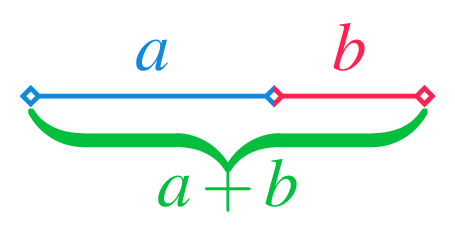
\includegraphics{././img/sucesiones/numero-aureo.png}

tal que \(\frac{a+b}{a}=\frac{a}{b}=\varphi\). A este número se le
conoce como
\href{https://es.wikipedia.org/wiki/N\%C3\%BAmero_\%C3\%A1ureo}{número
áureo} y es el número irracional
\(\varphi=\frac{1+\sqrt{5}}{2}=1.618033988749\ldots\)

Demostrar que este número es el límite de las siguientes sucesiones de
números reales.

\begin{enumerate}
\def\labelenumi{\alph{enumi}.}
\tightlist
\item
  \(x_1=1\) y \(x_{n+1}=1+\frac{1}{x_n}\) \(\forall n=1,2,\ldots\)
\item
  \(x_1=1\) y \(x_{n+1}=\sqrt{1+x_n}\) \(\forall n=1,2,\ldots\)
\end{enumerate}

\end{exercise}

\leavevmode\vadjust pre{\hypertarget{exr-sucesion-intereses}{}}%
\begin{exercise}[]\label{exr-sucesion-intereses}

Una cuenta de ahorro ofrece el primer año un tipo de interés
\(x_1=0.5\%\) y los años sucesivos un interés
\(x_{n+1}=\frac{3}{2+x_n}\). Si se mantiene la cuenta abierta por un
periodo indefinido, ¿hacia donde tienden los tipos de interés?

\end{exercise}

\leavevmode\vadjust pre{\hypertarget{exr-sucesiones-cauchy}{}}%
\begin{exercise}[]\label{exr-sucesiones-cauchy}

Determinar cuáles de las siguientes sucesiones de números reales son de
Cauchy.

\begin{enumerate}
\def\labelenumi{\alph{enumi}.}
\item
  \(\left(\frac{(-1)^n}{n}\right)_{n=1}^\infty\)
\item
  \(\left(\frac{n}{n+1}\right)_{n=1}^\infty\)
\item
  \(\left(\frac{\operatorname{sen}(n)}{n}\right)_{n=1}^\infty\)
\end{enumerate}

\end{exercise}



\end{document}
